% !TeX program = pdfLaTeX
\documentclass[12pt]{article}
\usepackage{amsmath}
\usepackage{graphicx,psfrag,epsf}
\usepackage{enumerate}
\usepackage{natbib}
\usepackage{textcomp}
\usepackage[hyphens]{url} % not crucial - just used below for the URL
\usepackage{hyperref}
\providecommand{\tightlist}{%
  \setlength{\itemsep}{0pt}\setlength{\parskip}{0pt}}

%\pdfminorversion=4
% NOTE: To produce blinded version, replace "0" with "1" below.
\newcommand{\blind}{0}

% DON'T change margins - should be 1 inch all around.
\addtolength{\oddsidemargin}{-.5in}%
\addtolength{\evensidemargin}{-.5in}%
\addtolength{\textwidth}{1in}%
\addtolength{\textheight}{1.3in}%
\addtolength{\topmargin}{-.8in}%

%% load any required packages here


\usepackage{color}
\usepackage{fancyvrb}
\newcommand{\VerbBar}{|}
\newcommand{\VERB}{\Verb[commandchars=\\\{\}]}
\DefineVerbatimEnvironment{Highlighting}{Verbatim}{commandchars=\\\{\}}
% Add ',fontsize=\small' for more characters per line
\usepackage{framed}
\definecolor{shadecolor}{RGB}{248,248,248}
\newenvironment{Shaded}{\begin{snugshade}}{\end{snugshade}}
\newcommand{\AlertTok}[1]{\textcolor[rgb]{0.94,0.16,0.16}{#1}}
\newcommand{\AnnotationTok}[1]{\textcolor[rgb]{0.56,0.35,0.01}{\textbf{\textit{#1}}}}
\newcommand{\AttributeTok}[1]{\textcolor[rgb]{0.77,0.63,0.00}{#1}}
\newcommand{\BaseNTok}[1]{\textcolor[rgb]{0.00,0.00,0.81}{#1}}
\newcommand{\BuiltInTok}[1]{#1}
\newcommand{\CharTok}[1]{\textcolor[rgb]{0.31,0.60,0.02}{#1}}
\newcommand{\CommentTok}[1]{\textcolor[rgb]{0.56,0.35,0.01}{\textit{#1}}}
\newcommand{\CommentVarTok}[1]{\textcolor[rgb]{0.56,0.35,0.01}{\textbf{\textit{#1}}}}
\newcommand{\ConstantTok}[1]{\textcolor[rgb]{0.00,0.00,0.00}{#1}}
\newcommand{\ControlFlowTok}[1]{\textcolor[rgb]{0.13,0.29,0.53}{\textbf{#1}}}
\newcommand{\DataTypeTok}[1]{\textcolor[rgb]{0.13,0.29,0.53}{#1}}
\newcommand{\DecValTok}[1]{\textcolor[rgb]{0.00,0.00,0.81}{#1}}
\newcommand{\DocumentationTok}[1]{\textcolor[rgb]{0.56,0.35,0.01}{\textbf{\textit{#1}}}}
\newcommand{\ErrorTok}[1]{\textcolor[rgb]{0.64,0.00,0.00}{\textbf{#1}}}
\newcommand{\ExtensionTok}[1]{#1}
\newcommand{\FloatTok}[1]{\textcolor[rgb]{0.00,0.00,0.81}{#1}}
\newcommand{\FunctionTok}[1]{\textcolor[rgb]{0.00,0.00,0.00}{#1}}
\newcommand{\ImportTok}[1]{#1}
\newcommand{\InformationTok}[1]{\textcolor[rgb]{0.56,0.35,0.01}{\textbf{\textit{#1}}}}
\newcommand{\KeywordTok}[1]{\textcolor[rgb]{0.13,0.29,0.53}{\textbf{#1}}}
\newcommand{\NormalTok}[1]{#1}
\newcommand{\OperatorTok}[1]{\textcolor[rgb]{0.81,0.36,0.00}{\textbf{#1}}}
\newcommand{\OtherTok}[1]{\textcolor[rgb]{0.56,0.35,0.01}{#1}}
\newcommand{\PreprocessorTok}[1]{\textcolor[rgb]{0.56,0.35,0.01}{\textit{#1}}}
\newcommand{\RegionMarkerTok}[1]{#1}
\newcommand{\SpecialCharTok}[1]{\textcolor[rgb]{0.00,0.00,0.00}{#1}}
\newcommand{\SpecialStringTok}[1]{\textcolor[rgb]{0.31,0.60,0.02}{#1}}
\newcommand{\StringTok}[1]{\textcolor[rgb]{0.31,0.60,0.02}{#1}}
\newcommand{\VariableTok}[1]{\textcolor[rgb]{0.00,0.00,0.00}{#1}}
\newcommand{\VerbatimStringTok}[1]{\textcolor[rgb]{0.31,0.60,0.02}{#1}}
\newcommand{\WarningTok}[1]{\textcolor[rgb]{0.56,0.35,0.01}{\textbf{\textit{#1}}}}


\usepackage{float} \floatplacement{figure}{H}
\usepackage{booktabs}
\usepackage{longtable}
\usepackage{array}
\usepackage{multirow}
\usepackage{wrapfig}
\usepackage{float}
\usepackage{colortbl}
\usepackage{pdflscape}
\usepackage{tabu}
\usepackage{threeparttable}
\usepackage{threeparttablex}
\usepackage[normalem]{ulem}
\usepackage{makecell}
\usepackage{xcolor}

\begin{document}


\def\spacingset#1{\renewcommand{\baselinestretch}%
{#1}\small\normalsize} \spacingset{1}


%%%%%%%%%%%%%%%%%%%%%%%%%%%%%%%%%%%%%%%%%%%%%%%%%%%%%%%%%%%%%%%%%%%%%%%%%%%%%%

\if0\blind
{
  \title{\bf MATH2269 Semester 2 2020 - Final Project}

  \author{
        Sam Holt, Phil Steinke, Elleni Toumpas \\
    RMIT\\
      }
  \maketitle
} \fi

\if1\blind
{
  \bigskip
  \bigskip
  \bigskip
  \begin{center}
    {\LARGE\bf MATH2269 Semester 2 2020 - Final Project}
  \end{center}
  \medskip
} \fi

\bigskip
\begin{abstract}
Insert Abstract
\end{abstract}

\noindent%
{\it Keywords:} JAGS, multiple linear regression analysis, prediction
\vfill

\newpage
\spacingset{1.45} % DON'T change the spacing!

\hypertarget{introduction}{%
\subsection{Introduction}\label{introduction}}

\hypertarget{analysis}{%
\subsection{Analysis}\label{analysis}}

\begin{Shaded}
\begin{Highlighting}[]
\NormalTok{data_cleaned <-}\StringTok{ }\NormalTok{data_cleaned }\OperatorTok\StringTok{ }
\StringTok{  }\KeywordTok{mutate}\NormalTok{(}\DataTypeTok{dow =} \KeywordTok{factor}\NormalTok{(dow, }\DataTypeTok{levels =} \KeywordTok{c}\NormalTok{(}\StringTok{'Monday'}\NormalTok{,}\StringTok{'Tuesday'}\NormalTok{,}\StringTok{'Wednesday'}\NormalTok{,}\StringTok{'Thursday'}\NormalTok{,}\StringTok{'Friday'}\NormalTok{,}\StringTok{'Saturday'}\NormalTok{,}\StringTok{'Sunday'}\NormalTok{), }
                           \DataTypeTok{labels =} \KeywordTok{c}\NormalTok{(}\StringTok{'Monday'}\NormalTok{,}\StringTok{'Tuesday'}\NormalTok{,}\StringTok{'Wednesday'}\NormalTok{,}\StringTok{'Thursday'}\NormalTok{,}\StringTok{'Friday'}\NormalTok{,}\StringTok{'Saturday'}\NormalTok{,}\StringTok{'Sunday'}\NormalTok{), }\DataTypeTok{ordered =} \OtherTok{TRUE}\NormalTok{), }
         \DataTypeTok{winddire =} \KeywordTok{factor}\NormalTok{(winddire, }
                           \DataTypeTok{levels =} \KeywordTok{c}\NormalTok{(}\StringTok{'N'}\NormalTok{, }\StringTok{'NNE'}\NormalTok{, }\StringTok{'NE'}\NormalTok{, }\StringTok{'ENE'}\NormalTok{, }\StringTok{'E'}\NormalTok{, }\StringTok{'ESE'}\NormalTok{, }\StringTok{'SE'}\NormalTok{, }\StringTok{'SSE'}\NormalTok{, }\StringTok{'S'}\NormalTok{, }\StringTok{'SSW'}\NormalTok{, }\StringTok{'SW'}\NormalTok{, }\StringTok{'WSW'}\NormalTok{, }\StringTok{'W'}\NormalTok{, }\StringTok{'WNW'}\NormalTok{, }\StringTok{'NW'}\NormalTok{,}\StringTok{'NNW'}\NormalTok{), }
                           \DataTypeTok{labels =} \KeywordTok{c}\NormalTok{(}\StringTok{'N'}\NormalTok{, }\StringTok{'NNE'}\NormalTok{, }\StringTok{'NE'}\NormalTok{, }\StringTok{'ENE'}\NormalTok{, }\StringTok{'E'}\NormalTok{, }\StringTok{'ESE'}\NormalTok{, }\StringTok{'SE'}\NormalTok{, }\StringTok{'SSE'}\NormalTok{, }\StringTok{'S'}\NormalTok{, }\StringTok{'SSW'}\NormalTok{, }\StringTok{'SW'}\NormalTok{, }\StringTok{'WSW'}\NormalTok{, }\StringTok{'W'}\NormalTok{, }\StringTok{'WNW'}\NormalTok{, }\StringTok{'NW'}\NormalTok{,}\StringTok{'NNW'}\NormalTok{),}
                           \DataTypeTok{ordered =} \OtherTok{TRUE}\NormalTok{))}
\end{Highlighting}
\end{Shaded}

\hypertarget{a-descriptive-look}{%
\subsubsection{A descriptive look}\label{a-descriptive-look}}

\hypertarget{dimensions}{%
\paragraph{Dimensions}\label{dimensions}}

\begin{longtable}[]{@{}rr@{}}
\caption{Dimenions}\tabularnewline
\toprule
columns & rows\tabularnewline
\midrule
\endfirsthead
\toprule
columns & rows\tabularnewline
\midrule
\endhead
28 & 25626\tabularnewline
\bottomrule
\end{longtable}

\begin{landscape}\begin{table}

\caption{\label{tab:unnamed-chunk-3}Inspecting the first six rows of the data.}
\centering
\fontsize{6}{8}\selectfont
\begin{tabu} to \linewidth {>{\raggedleft}X>{\raggedright}X>{\raggedleft}X>{\raggedright}X>{\raggedright}X>{\raggedright}X>{\raggedright}X>{\raggedright}X>{\raggedright}X}
\hline
\rotatebox{90}{years} & \rotatebox{90}{yn80} & \rotatebox{90}{roll\_temp} & \rotatebox{90}{yn50} & \rotatebox{90}{north} & \rotatebox{90}{north1} & \rotatebox{90}{yn60} & \rotatebox{90}{weekdays} & \rotatebox{90}{mornings}\\
\hline
2016 & FALSE & NA & FALSE & FALSE & FALSE & FALSE & TRUE & FALSE\\
\hline
2016 & FALSE & NA & FALSE & TRUE & FALSE & FALSE & TRUE & \vphantom{1} FALSE\\
\hline
2016 & FALSE & NA & FALSE & TRUE & FALSE & FALSE & TRUE & FALSE\\
\hline
2016 & FALSE & NA & FALSE & TRUE & TRUE & FALSE & TRUE & \vphantom{1} FALSE\\
\hline
2016 & FALSE & NA & FALSE & TRUE & TRUE & FALSE & TRUE & FALSE\\
\hline
\end{tabu}
\end{table}
\end{landscape}

\hypertarget{datatypes}{%
\paragraph{Datatypes}\label{datatypes}}

The datatypes for each variable can be found below (after variable
datatypes were set on import). Numerical variables that are actually
binary values or an identifier were transformed to a factor.

\begin{table}

\caption{\label{tab:unnamed-chunk-4}Data types}
\centering
\begin{tabu} to \linewidth {>{\raggedright}X>{\raggedright}X>{\raggedright}X}
\hline
  & class & NA\\
\hline
id & numeric & numeric\\
\hline
rainfall\_mm & numeric & numeric\\
\hline
rf\_cum\_2\_day & numeric & numeric\\
\hline
rf\_cum\_3\_day & numeric & numeric\\
\hline
rf\_cum\_4\_day & numeric & numeric\\
\hline
rf\_cum\_5\_day & numeric & numeric\\
\hline
rf\_cum\_6\_day & numeric & numeric\\
\hline
rf\_cum\_7\_day & numeric & numeric\\
\hline
date\_day & Date & Date\\
\hline
date\_local\_time & POSIXct POSIXt & POSIXct POSIXt\\
\hline
site & character & character\\
\hline
temperature & numeric & numeric\\
\hline
pm10 & numeric & numeric\\
\hline
pm10a & numeric & numeric\\
\hline
wd & numeric & numeric\\
\hline
ws & numeric & numeric\\
\hline
dow & ordered & factor\\
\hline
hour & numeric & numeric\\
\hline
winddire & ordered & factor\\
\hline
years & numeric & numeric\\
\hline
yn80 & logical & logical\\
\hline
roll\_temp & numeric & numeric\\
\hline
yn50 & logical & logical\\
\hline
north & logical & logical\\
\hline
north1 & logical & logical\\
\hline
yn60 & logical & logical\\
\hline
weekdays & logical & logical\\
\hline
mornings & logical & logical\\
\hline
\end{tabu}
\end{table}

\hypertarget{data-preprocessing}{%
\paragraph{Data Preprocessing}\label{data-preprocessing}}

\hypertarget{removing-unique-identifier}{%
\subparagraph{Removing unique
identifier}\label{removing-unique-identifier}}

\begin{table}

\caption{\label{tab:unnamed-chunk-5}The count of id variable filtered to show only values that are not unique.}
\centering
\begin{tabu} to \linewidth {>{\raggedleft}X>{\raggedleft}X}
\hline
id & count\\


\hline
\end{tabu}
\end{table}

As confirmed above, the \textbf{id} is a unique identifier, and it is
therefore removed from the dataset.

Regarding the other variables removed, we have determined \(PM_{10}\) as
our target variable, the remain proposed target variables
(\(PM_{10}a, yn_{80}, yn_{60}, yn_{50}\)) are therfore discarded.

\hypertarget{outliers}{%
\subparagraph{Outliers}\label{outliers}}

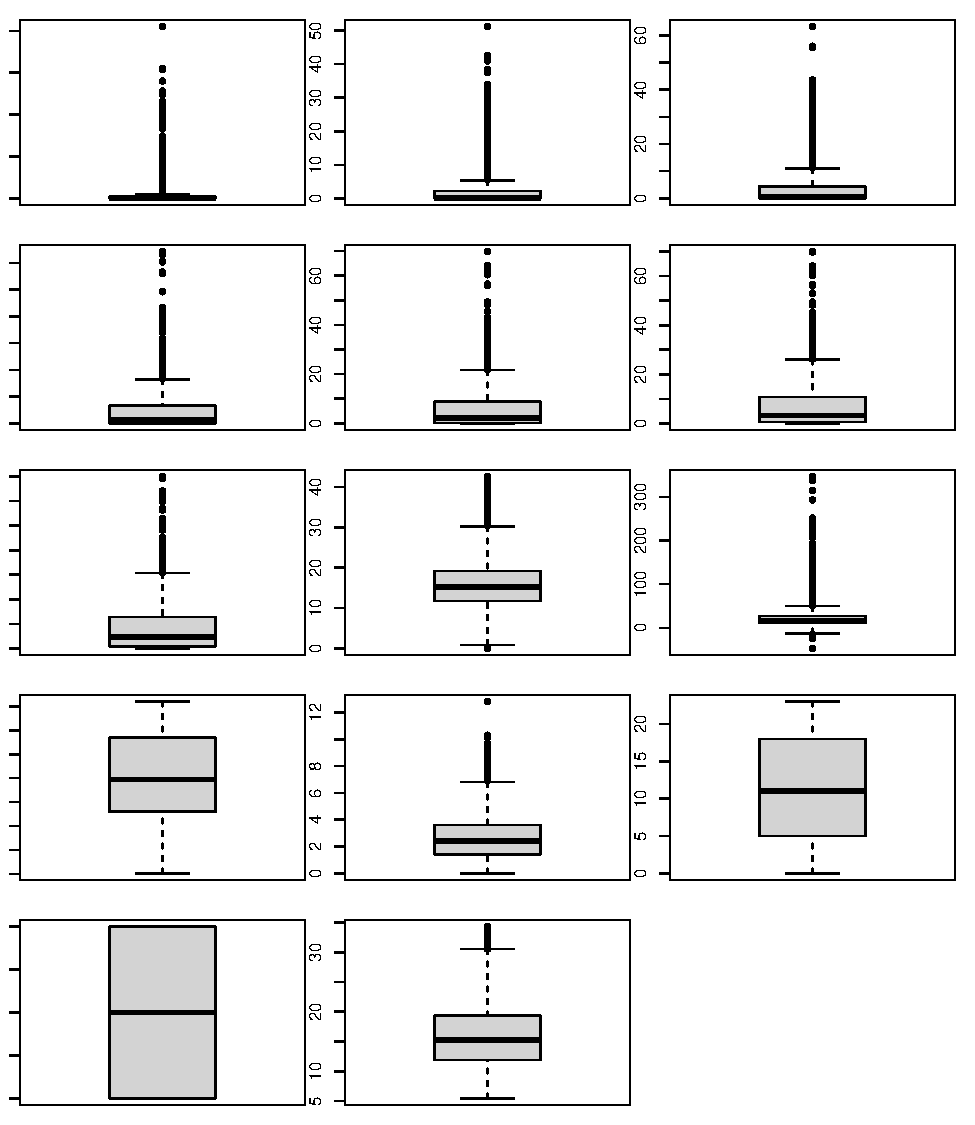
\includegraphics{MATH2269_final_project_files/figure-latex/unnamed-chunk-8-1.pdf}

\hypertarget{impossible-values}{%
\subparagraph{Impossible values}\label{impossible-values}}

For the numerical values in the dataset an impossible value check is
performed.

\begin{table}

\caption{\label{tab:unnamed-chunk-9}The number of rows with impossible values.}
\centering
\begin{tabu} to \linewidth {>{\raggedright}X>{\raggedleft}X}
\hline
column & nrows\\
\hline
rainfall\_mm & 0\\
\hline
rf\_cum\_2\_day & 0\\
\hline
rf\_cum\_3\_day & 0\\
\hline
rf\_cum\_4\_day & 0\\
\hline
rf\_cum\_5\_day & 0\\
\hline
rf\_cum\_6\_day & 0\\
\hline
rf\_cum\_7\_day & 0\\
\hline
rf\_cum\_5\_day & 0\\
\hline
date\_day & 0\\
\hline
temperature & 0\\
\hline
pm10 & 118\\
\hline
wd & 0\\
\hline
ws & 0\\
\hline
hour & 0\\
\hline
years & 0\\
\hline
roll\_temp & 0\\
\hline
\end{tabu}
\end{table}

\hypertarget{missing-values}{%
\subparagraph{Missing values}\label{missing-values}}

Checking the missing values we can see that there are 23 rolling
temperate missing records.

\begin{table}

\caption{\label{tab:unnamed-chunk-10}Count of missing values by variable}
\centering
\begin{tabu} to \linewidth {>{\raggedright}X>{\raggedleft}X}
\hline
  & Number missing values\\
\hline
rainfall\_mm & 0\\
\hline
rf\_cum\_2\_day & 0\\
\hline
rf\_cum\_3\_day & 0\\
\hline
rf\_cum\_4\_day & 0\\
\hline
rf\_cum\_5\_day & 0\\
\hline
rf\_cum\_6\_day & 0\\
\hline
rf\_cum\_7\_day & 0\\
\hline
date\_day & 0\\
\hline
date\_local\_time & 0\\
\hline
site & 0\\
\hline
temperature & 0\\
\hline
pm10 & 0\\
\hline
wd & 0\\
\hline
ws & 0\\
\hline
dow & 0\\
\hline
hour & 0\\
\hline
winddire & 0\\
\hline
years & 0\\
\hline
roll\_temp & 23\\
\hline
north & 0\\
\hline
north1 & 0\\
\hline
weekdays & 0\\
\hline
mornings & 0\\
\hline
\end{tabu}
\end{table}

\begin{Shaded}
\begin{Highlighting}[]
\NormalTok{data_cleaned }\OperatorTok
\StringTok{  }\KeywordTok{filter}\NormalTok{(}\KeywordTok{is.na}\NormalTok{(roll_temp)) }\OperatorTok
\StringTok{  }\KeywordTok{select}\NormalTok{(date_day, date_local_time, roll_temp, pm10) }\OperatorTok
\StringTok{  }\KeywordTok{format_table}\NormalTok{(}\DataTypeTok{p_caption =} \StringTok{"Missing roll temperate values"}\NormalTok{)}
\end{Highlighting}
\end{Shaded}

\begin{table}

\caption{\label{tab:unnamed-chunk-11}Missing roll temperate values}
\centering
\begin{tabu} to \linewidth {>{\raggedright}X>{\raggedright}X>{\raggedleft}X>{\raggedleft}X}
\hline
date\_day & date\_local\_time & roll\_temp & pm10\\
\hline
2016-01-01 & 2016-01-01 00:00:00 & NA & 30.5\\
\hline
2016-01-01 & 2016-01-01 01:00:00 & NA & 25.8\\
\hline
2016-01-01 & 2016-01-01 02:00:00 & NA & 22.2\\
\hline
2016-01-01 & 2016-01-01 03:00:00 & NA & 23.2\\
\hline
2016-01-01 & 2016-01-01 04:00:00 & NA & 24.3\\
\hline
2016-01-01 & 2016-01-01 05:00:00 & NA & 33.4\\
\hline
2016-01-01 & 2016-01-01 06:00:00 & NA & 35.3\\
\hline
2016-01-01 & 2016-01-01 07:00:00 & NA & 29.6\\
\hline
2016-01-01 & 2016-01-01 08:00:00 & NA & 45.1\\
\hline
2016-01-01 & 2016-01-01 09:00:00 & NA & 22.6\\
\hline
2016-01-01 & 2016-01-01 10:00:00 & NA & 18.8\\
\hline
2018-12-31 & 2018-12-31 12:00:00 & NA & 32.6\\
\hline
2018-12-31 & 2018-12-31 13:00:00 & NA & 25.9\\
\hline
2018-12-31 & 2018-12-31 14:00:00 & NA & 30.1\\
\hline
2018-12-31 & 2018-12-31 15:00:00 & NA & 21.6\\
\hline
2018-12-31 & 2018-12-31 16:00:00 & NA & 17.5\\
\hline
2018-12-31 & 2018-12-31 17:00:00 & NA & 19.2\\
\hline
2018-12-31 & 2018-12-31 18:00:00 & NA & 20.9\\
\hline
2018-12-31 & 2018-12-31 19:00:00 & NA & 22.2\\
\hline
2018-12-31 & 2018-12-31 20:00:00 & NA & 8.9\\
\hline
2018-12-31 & 2018-12-31 21:00:00 & NA & 5.1\\
\hline
2018-12-31 & 2018-12-31 22:00:00 & NA & 3.1\\
\hline
2018-12-31 & 2018-12-31 23:00:00 & NA & 10.5\\
\hline
\end{tabu}
\end{table}

It is therefore sufficient to simply remove these records from the
dataset.

\begin{Shaded}
\begin{Highlighting}[]
\CommentTok{# Remove incomplete rows}
\NormalTok{data_cleaned <-}\StringTok{ }\NormalTok{data_cleaned[}\KeywordTok{complete.cases}\NormalTok{(data_cleaned),]}
\end{Highlighting}
\end{Shaded}

\hypertarget{feature-engineering}{%
\subparagraph{Feature engineering}\label{feature-engineering}}

\begin{Shaded}
\begin{Highlighting}[]
\CommentTok{# Do we need to create any new features from the data set?}
\end{Highlighting}
\end{Shaded}

\hypertarget{categorical-features}{%
\subparagraph{Categorical Features}\label{categorical-features}}

To check whether there are errors (including typos or unexpected values)
in the categorical features each variable is arranged in order and then
inspected by the researchers. In the list of possible values printed
below there seems to be no incorrect values.

\begin{Shaded}
\begin{Highlighting}[]
\ControlFlowTok{for}\NormalTok{ (col }\ControlFlowTok{in} \KeywordTok{colnames}\NormalTok{(data_cleaned)) \{}
  
  \ControlFlowTok{if}\NormalTok{ (}\KeywordTok{class}\NormalTok{(data_cleaned[[col]])[}\DecValTok{1}\NormalTok{] }\OperatorTok\StringTok{ }\KeywordTok{c}\NormalTok{(}\StringTok{'factor'}\NormalTok{, }\StringTok{'ordered'}\NormalTok{, }\StringTok{'character'}\NormalTok{)) \{}

    \KeywordTok{paste0}\NormalTok{(}\StringTok{"Unique values for "}\NormalTok{,col) }\OperatorTok\StringTok{ }\KeywordTok{cat}\NormalTok{()}
    \KeywordTok{cat}\NormalTok{(}\StringTok{"}\CharTok{\textbackslash{}n}\StringTok{"}\NormalTok{)}

\NormalTok{    data_cleaned }\OperatorTok
\StringTok{      }\KeywordTok{arrange}\NormalTok{(}\KeywordTok{get}\NormalTok{(col)) }\OperatorTok
\StringTok{      }\KeywordTok{select}\NormalTok{(col) }\OperatorTok
\StringTok{      }\KeywordTok{unique}\NormalTok{() }\OperatorTok
\StringTok{      }\KeywordTok{pull}\NormalTok{() }\OperatorTok
\StringTok{      }\KeywordTok{as.character}\NormalTok{() }\OperatorTok
\StringTok{      }\KeywordTok{paste0}\NormalTok{(}\DataTypeTok{collapse =} \StringTok{", "}\NormalTok{) }\OperatorTok
\StringTok{      }\NormalTok{stringr}\OperatorTok{::}\KeywordTok{str_trunc}\NormalTok{(}\DataTypeTok{width =} \DecValTok{800}\NormalTok{, }\DataTypeTok{side =} \StringTok{"right"}\NormalTok{, }\DataTypeTok{ellipsis =} \StringTok{"... (truncated)"}\NormalTok{) }\OperatorTok
\StringTok{      }\KeywordTok{cat}\NormalTok{()}

    \KeywordTok{cat}\NormalTok{(}\StringTok{"}\CharTok{\textbackslash{}n}\StringTok{"}\NormalTok{)}
    \KeywordTok{cat}\NormalTok{(}\StringTok{"}\CharTok{\textbackslash{}n}\StringTok{"}\NormalTok{)}

\NormalTok{  \}}
\NormalTok{\}}
\end{Highlighting}
\end{Shaded}

\begin{verbatim}
## Unique values for site
## Brooklyn
## 
## Unique values for dow
## Monday, Tuesday, Wednesday, Thursday, Friday, Saturday, Sunday
## 
## Unique values for winddire
## N, NNE, NE, ENE, E, ESE, SE, SSE, S, SSW, SW, WSW, W, WNW, NW, NNW
\end{verbatim}

\hypertarget{any-categorical-descriptive-feature-encoded}{%
\subparagraph{Any categorical descriptive feature
encoded}\label{any-categorical-descriptive-feature-encoded}}

\begin{Shaded}
\begin{Highlighting}[]
\CommentTok{### Do we need to encode categorical variables?}

\CommentTok{## Make sure we have these columns in or captured in the dataset....}
\CommentTok{# Rain 3 day}
\CommentTok{# Temperature}
\CommentTok{# WD}
\CommentTok{# WS}
\CommentTok{# day of the week}
\CommentTok{# week day/ work day/ public holiday/ weekends}
\CommentTok{# 24 hour clock hour}
\CommentTok{# change wind direction into degrees from north}

\NormalTok{holidays <-}\StringTok{ }\NormalTok{tsibble}\OperatorTok{::}\KeywordTok{holiday_aus}\NormalTok{(}\KeywordTok{unique}\NormalTok{(data_cleaned}\OperatorTok{$}\NormalTok{years), }\DataTypeTok{state =} \StringTok{'VIC'}\NormalTok{)}

\NormalTok{data_cleaned <-}\StringTok{ }\NormalTok{data_cleaned }\OperatorTok
\StringTok{  }\KeywordTok{mutate}\NormalTok{(}
    \DataTypeTok{deg_from_north =} \KeywordTok{case_when}\NormalTok{(}
\NormalTok{      wd }\OperatorTok{>}\StringTok{ }\DecValTok{180} \OperatorTok{~}\StringTok{ }\KeywordTok{abs}\NormalTok{(wd }\OperatorTok{-}\StringTok{ }\DecValTok{360}\NormalTok{),}
      \OtherTok{TRUE} \OperatorTok{~}\StringTok{ }\NormalTok{wd}
\NormalTok{    ),}
    \DataTypeTok{pre_peak_hour =} \KeywordTok{case_when}\NormalTok{(}
\NormalTok{      hour }\OperatorTok{>}\StringTok{ }\DecValTok{4} \OperatorTok{&}\StringTok{ }\NormalTok{hour }\OperatorTok{<}\StringTok{ }\DecValTok{9} \OperatorTok{~}\StringTok{ }\OtherTok{TRUE}\NormalTok{,}
\NormalTok{      hour }\OperatorTok{>}\StringTok{ }\DecValTok{14} \OperatorTok{&}\StringTok{ }\NormalTok{hour }\OperatorTok{<}\StringTok{ }\DecValTok{17} \OperatorTok{~}\StringTok{ }\OtherTok{TRUE}\NormalTok{,}
      \OtherTok{TRUE} \OperatorTok{~}\StringTok{ }\OtherTok{FALSE}
\NormalTok{    ),}
    \DataTypeTok{working_days =} \KeywordTok{case_when}\NormalTok{(}
\NormalTok{      weekdays }\OperatorTok{==}\StringTok{ }\OtherTok{TRUE} \OperatorTok{~}\StringTok{ }\OtherTok{TRUE}\NormalTok{,}
\NormalTok{      date_day }\OperatorTok\StringTok{ }\NormalTok{holidays}\OperatorTok{$}\NormalTok{date }\OperatorTok{~}\StringTok{ }\OtherTok{FALSE}\NormalTok{,}
\NormalTok{      weekdays }\OperatorTok{==}\StringTok{ }\OtherTok{FALSE} \OperatorTok{~}\StringTok{ }\OtherTok{FALSE}
\NormalTok{    )}
\NormalTok{  )}

\CommentTok{# Base sanity checks}
\KeywordTok{summary}\NormalTok{(data_cleaned}\OperatorTok{$}\NormalTok{deg_from_north)}
\end{Highlighting}
\end{Shaded}

\begin{verbatim}
##    Min. 1st Qu.  Median    Mean 3rd Qu.    Max. 
##    0.00   23.00   86.00   86.99  151.00  180.00
\end{verbatim}

\begin{Shaded}
\begin{Highlighting}[]
\NormalTok{data_cleaned }\OperatorTok\StringTok{ }\KeywordTok{count}\NormalTok{(hour, pre_peak_hour)}
\end{Highlighting}
\end{Shaded}

\begin{verbatim}
## # A tibble: 24 x 3
##     hour pre_peak_hour     n
##    <dbl> <lgl>         <int>
##  1     0 FALSE          1076
##  2     1 FALSE          1069
##  3     2 FALSE          1070
##  4     3 FALSE          1069
##  5     4 FALSE          1071
##  6     5 TRUE           1074
##  7     6 TRUE           1072
##  8     7 TRUE           1069
##  9     8 TRUE           1072
## 10     9 FALSE          1067
## # ... with 14 more rows
\end{verbatim}

\begin{Shaded}
\begin{Highlighting}[]
\NormalTok{data_cleaned }\OperatorTok\StringTok{ }\KeywordTok{count}\NormalTok{(working_days)}
\end{Highlighting}
\end{Shaded}

\begin{verbatim}
## # A tibble: 2 x 2
##   working_days     n
##   <lgl>        <int>
## 1 FALSE         7425
## 2 TRUE         18178
\end{verbatim}

If we were to have issues within the pre\_peak\_hour summary, there
would either be a duplicate of the hour values or NA values in both hour
and pre\_peak\_hour fields.

\hypertarget{summary-statistics}{%
\subparagraph{Summary statistics}\label{summary-statistics}}

A quick look at the custom summary statistics can be found below. For
factors we can see the most common level, with the count of appearances
for that mode level. For the Date variables we can we can see the min,
max and mode levels. For the numeric and integer variables we can see
the mean, median, standard deviation, minimum and maximum values.

\begin{Shaded}
\begin{Highlighting}[]
\NormalTok{results_df <-}\StringTok{ }\KeywordTok{exploratory_summarize}\NormalTok{(data_cleaned, col }\OperatorTok{==}\StringTok{ 'id'}\NormalTok{)}
\NormalTok{results_df }\OperatorTok\StringTok{  }\KeywordTok{format_table}\NormalTok{(}\DataTypeTok{p_caption =} \StringTok{"Exploratory dataset"}\NormalTok{)}
\end{Highlighting}
\end{Shaded}

\begin{table}

\caption{\label{tab:unnamed-chunk-16}Exploratory dataset}
\centering
\begin{tabu} to \linewidth {>{\raggedright}X>{\raggedright}X>{\raggedright}X>{\raggedright}X>{\raggedright}X>{\raggedright}X>{\raggedright}X>{\raggedright}X>{\raggedright}X>{\raggedright}X}
\hline
name & type & missing\_values & mean & median & sd & mode & min & max & nlevs\\
\hline
rainfall\_mm & numeric & 0 & 1.328 & 0 & 3.872 & NA & 0 & 41 & NA\\
\hline
rf\_cum\_2\_day & numeric & 0 & 2.654 & 0.2 & 5.997 & NA & 0 & 51.2 & NA\\
\hline
rf\_cum\_3\_day & numeric & 0 & 3.95 & 0.6 & 7.611 & NA & 0 & 63.2 & NA\\
\hline
rf\_cum\_4\_day & numeric & 0 & 5.245 & 1.4 & 8.928 & NA & 0 & 64.2 & NA\\
\hline
rf\_cum\_5\_day & numeric & 0 & 6.547 & 2.4 & 10.049 & NA & 0 & 69.8 & NA\\
\hline
rf\_cum\_6\_day & numeric & 0 & 7.863 & 3.2 & 11.055 & NA & 0 & 70 & NA\\
\hline
rf\_cum\_7\_day & numeric & 0 & 9.194 & 4.6 & 11.97 & NA & 0 & 70 & NA\\
\hline
date\_day & Date & 0 & NA & NA & NA & 2018-10-16 & 2016-01-01 & 2018-12-31 & NA\\
\hline
date\_local\_time & POSIXct & 0 & NA & NA & NA & NA & NA & NA & NA\\
\hline
date\_local\_time & POSIXt & 0 & NA & NA & NA & NA & NA & NA & NA\\
\hline
site & character & 0 & NA & NA & NA & NA & NA & NA & NA\\
\hline
temperature & numeric & 0 & 15.882 & 15.3 & 5.783 & NA & 0 & 42.6 & NA\\
\hline
pm10 & numeric & 0 & 22.325 & 16.9 & 19.712 & NA & -46.9000015259 & 346.2 & NA\\
\hline
wd & numeric & 0 & 193.784 & 197 & 110.883 & NA & 1 & 360 & NA\\
\hline
ws & numeric & 0 & 2.633 & 2.4 & 1.499 & NA & 0 & 12.8000001907 & NA\\
\hline
dow & ordered & 0 & NA & NA & NA & NA & NA & NA & NA\\
\hline
dow & factor & 0 & NA & NA & NA & NA & NA & NA & NA\\
\hline
hour & numeric & 0 & 11.491 & 11 & 6.933 & NA & 0 & 23 & NA\\
\hline
winddire & ordered & 0 & NA & NA & NA & NA & NA & NA & NA\\
\hline
winddire & factor & 0 & NA & NA & NA & NA & NA & NA & NA\\
\hline
years & numeric & 0 & 2017 & 2017 & 0.818 & NA & 2016 & 2018 & NA\\
\hline
roll\_temp & numeric & 0 & 15.882 & 15.213 & 4.926 & NA & 5.4500000079 & 34.2958333333 & NA\\
\hline
north & logical & 0 & NA & NA & NA & NA & NA & NA & NA\\
\hline
north1 & logical & 0 & NA & NA & NA & NA & NA & NA & NA\\
\hline
weekdays & logical & 0 & NA & NA & NA & NA & NA & NA & NA\\
\hline
mornings & logical & 0 & NA & NA & NA & NA & NA & NA & NA\\
\hline
deg\_from\_north & numeric & 0 & 86.986 & 86 & 61.912 & NA & 0 & 180 & NA\\
\hline
pre\_peak\_hour & logical & 0 & NA & NA & NA & NA & NA & NA & NA\\
\hline
working\_days & logical & 0 & NA & NA & NA & NA & NA & NA & NA\\
\hline
\end{tabu}
\end{table}

\hypertarget{univariate-distribution}{%
\subparagraph{Univariate distribution}\label{univariate-distribution}}

\begin{Shaded}
\begin{Highlighting}[]
\NormalTok{plots <-}\StringTok{ }\KeywordTok{list}\NormalTok{()}

\ControlFlowTok{for}\NormalTok{ (col }\ControlFlowTok{in} \KeywordTok{colnames}\NormalTok{(data_cleaned)) \{}
\NormalTok{  plots[[col]] <-}\StringTok{ }\KeywordTok{univariate_distribution_plot}\NormalTok{(data_cleaned[[col]], col)}
\NormalTok{\}}
\end{Highlighting}
\end{Shaded}

\begin{verbatim}
## [1] "date_local_time couldn't be plotted."
## [1] "site couldn't be plotted."
## [1] "north couldn't be plotted."
## [1] "north1 couldn't be plotted."
## [1] "weekdays couldn't be plotted."
## [1] "mornings couldn't be plotted."
## [1] "pre_peak_hour couldn't be plotted."
## [1] "working_days couldn't be plotted."
\end{verbatim}

\begin{Shaded}
\begin{Highlighting}[]
\KeywordTok{grid.arrange}\NormalTok{(}\DataTypeTok{grobs =}\NormalTok{ plots, }\DataTypeTok{ncol =} \DecValTok{3}\NormalTok{)}
\end{Highlighting}
\end{Shaded}

\begin{figure}
\centering
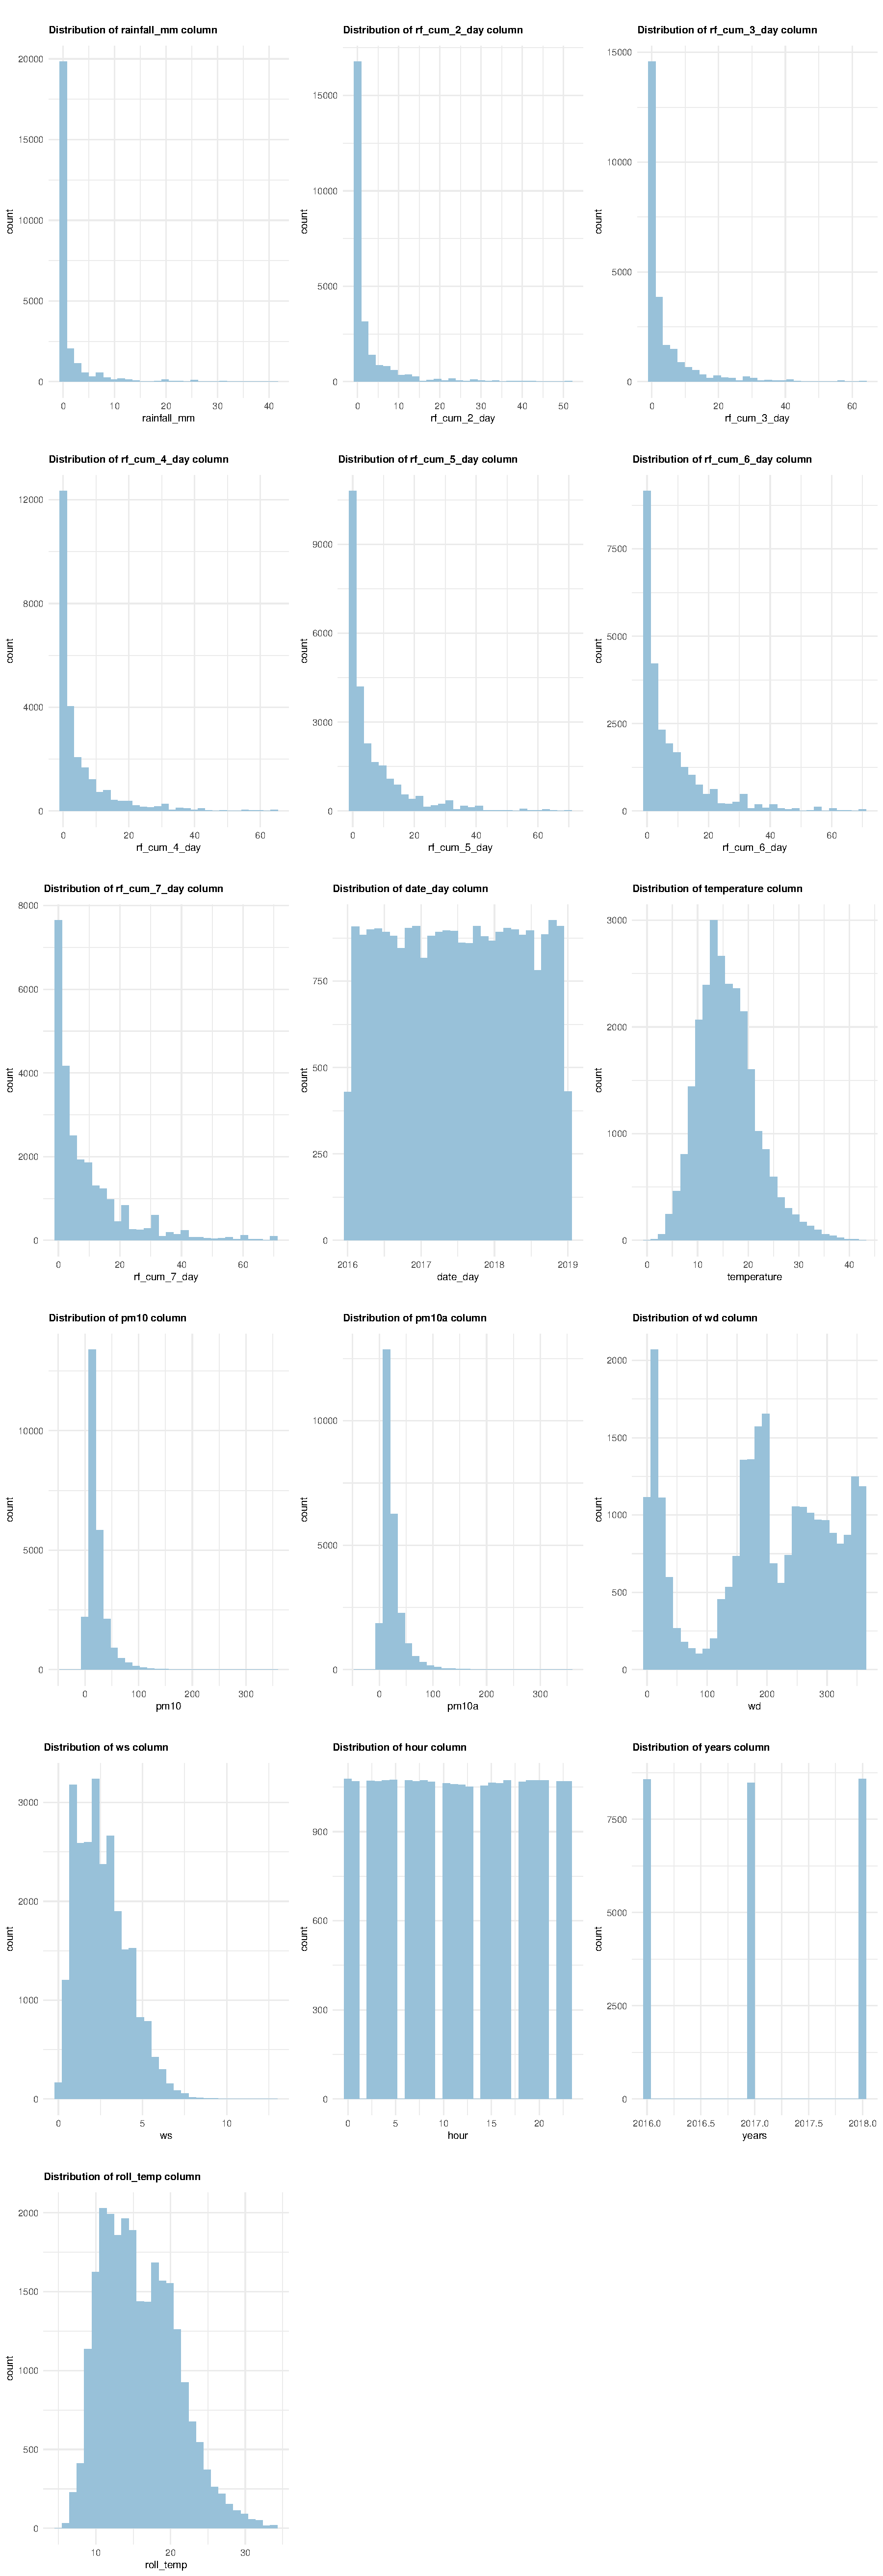
\includegraphics{MATH2269_final_project_files/figure-latex/Univariate distribution-1.pdf}
\caption{A univariate look at the distribution of all the variables
found in the Air dataset.}
\end{figure}

\begin{Shaded}
\begin{Highlighting}[]
\NormalTok{scatter_plots <-}\StringTok{ }\KeywordTok{list}\NormalTok{()}

\ControlFlowTok{for}\NormalTok{(col }\ControlFlowTok{in} \KeywordTok{colnames}\NormalTok{(data_cleaned))\{}
  \ControlFlowTok{if}\NormalTok{((}\KeywordTok{class}\NormalTok{(data_cleaned[[col]])[}\DecValTok{1}\NormalTok{] }\OperatorTok\StringTok{ }\KeywordTok{c}\NormalTok{(}\StringTok{'numeric'}\NormalTok{,}\StringTok{'integer'}\NormalTok{)) }\OperatorTok{&}\StringTok{ }\NormalTok{(col }\OperatorTok{!=}\StringTok{ 'pm10'}\NormalTok{))\{}
\NormalTok{    scatter_plots[[col]] <-}\StringTok{ }\KeywordTok{ggplot}\NormalTok{(data_cleaned, }\KeywordTok{aes_string}\NormalTok{(}\DataTypeTok{x =}\NormalTok{ col, }\DataTypeTok{y =} \StringTok{'pm10'}\NormalTok{)) }\OperatorTok{+}\StringTok{ }
\StringTok{      }\KeywordTok{geom_point}\NormalTok{(}\DataTypeTok{fill =} \StringTok{'orange'}\NormalTok{, }\DataTypeTok{alpha =} \FloatTok{0.3}\NormalTok{, }\DataTypeTok{col =} \StringTok{'orange'}\NormalTok{) }\OperatorTok{+}\StringTok{ }
\StringTok{      }\KeywordTok{labs}\NormalTok{(}\DataTypeTok{title =} \KeywordTok{paste0}\NormalTok{(col,}\StringTok{" plotted}\CharTok{\textbackslash{}n}\StringTok{against PM10 levels"}\NormalTok{)) }\OperatorTok{+}
\StringTok{      }\NormalTok{assignment_multi_plot_theme}
\NormalTok{  \}}
\NormalTok{\}}

\KeywordTok{grid.arrange}\NormalTok{(}\DataTypeTok{grobs =}\NormalTok{ scatter_plots, }\DataTypeTok{ncol =} \DecValTok{3}\NormalTok{)}
\end{Highlighting}
\end{Shaded}

\begin{figure}
\centering
\includegraphics{MATH2269_final_project_files/figure-latex/A numeric univariate vs target class distribution-1.pdf}
\caption{A}
\end{figure}

\begin{Shaded}
\begin{Highlighting}[]
\NormalTok{box_plots <-}\StringTok{ }\KeywordTok{list}\NormalTok{()}

\ControlFlowTok{for}\NormalTok{(col }\ControlFlowTok{in} \KeywordTok{colnames}\NormalTok{(data_cleaned))\{}
  \ControlFlowTok{if}\NormalTok{((}\KeywordTok{class}\NormalTok{(data_cleaned[[col]])[}\DecValTok{1}\NormalTok{] }\OperatorTok\StringTok{ }\KeywordTok{c}\NormalTok{(}\StringTok{'ordered'}\NormalTok{,}\StringTok{'factor'}\NormalTok{, }\StringTok{'character'}\NormalTok{, }\StringTok{'logical'}\NormalTok{)) }\OperatorTok{&}\StringTok{ }\NormalTok{(col }\OperatorTok{!=}\StringTok{ 'pm10'}\NormalTok{))\{}
    
\NormalTok{    box_plots[[col]] <-}\StringTok{ }\KeywordTok{ggplot}\NormalTok{(data_cleaned, }\KeywordTok{aes_string}\NormalTok{(}\DataTypeTok{x =}\NormalTok{ col, }\DataTypeTok{y =} \StringTok{'pm10'}\NormalTok{)) }\OperatorTok{+}\StringTok{ }
\StringTok{      }\KeywordTok{geom_boxplot}\NormalTok{(}\DataTypeTok{fill =} \StringTok{'orange'}\NormalTok{, }\DataTypeTok{alpha =} \FloatTok{0.3}\NormalTok{, }\DataTypeTok{col =} \StringTok{'orange'}\NormalTok{) }\OperatorTok{+}\StringTok{ }
\StringTok{      }\KeywordTok{labs}\NormalTok{(}\DataTypeTok{title =} \KeywordTok{paste0}\NormalTok{(col,}\StringTok{" plotted}\CharTok{\textbackslash{}n}\StringTok{against PM10 levels"}\NormalTok{)) }\OperatorTok{+}
\StringTok{      }\NormalTok{assignment_multi_plot_theme}
    
\NormalTok{  \} }
\NormalTok{\}}

\KeywordTok{grid.arrange}\NormalTok{(}\DataTypeTok{grobs =}\NormalTok{ box_plots, }\DataTypeTok{ncol =} \DecValTok{3}\NormalTok{)}
\end{Highlighting}
\end{Shaded}

\begin{figure}
\centering
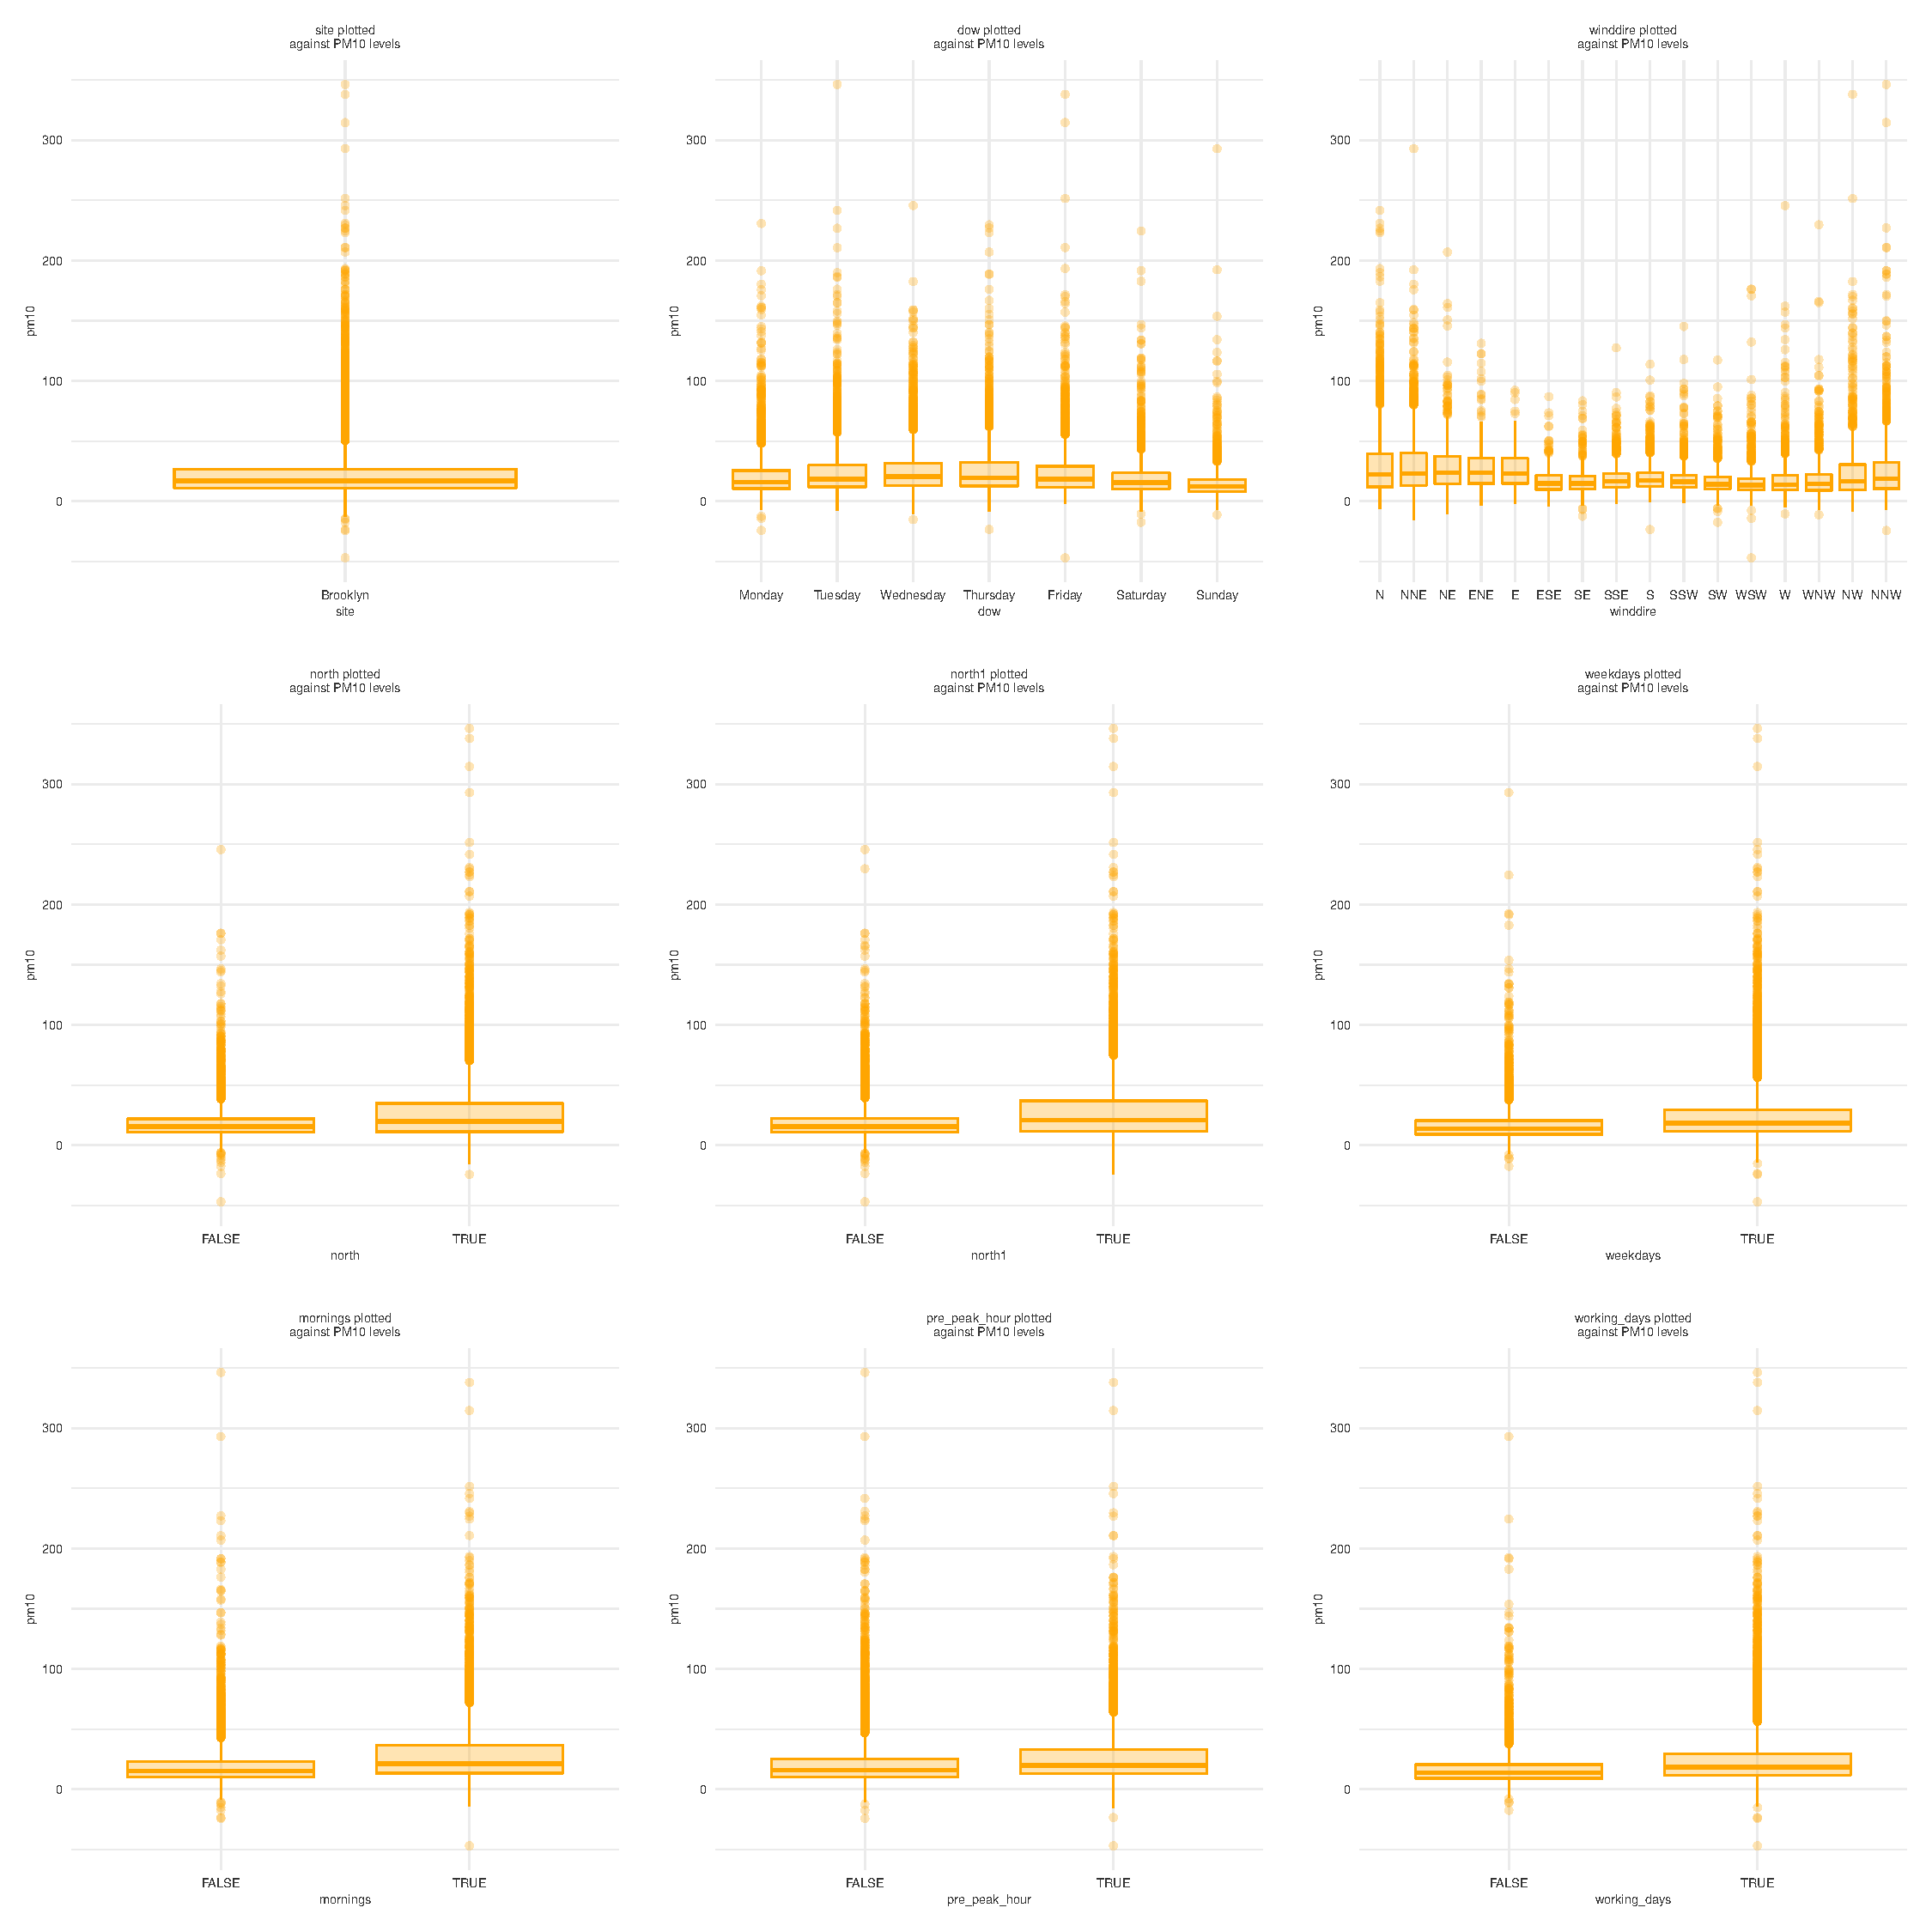
\includegraphics{MATH2269_final_project_files/figure-latex/A categorical univariate vs target class distribution-1.pdf}
\caption{A}
\end{figure}

\hypertarget{likelihood}{%
\paragraph{Likelihood}\label{likelihood}}

\begin{figure}
\centering
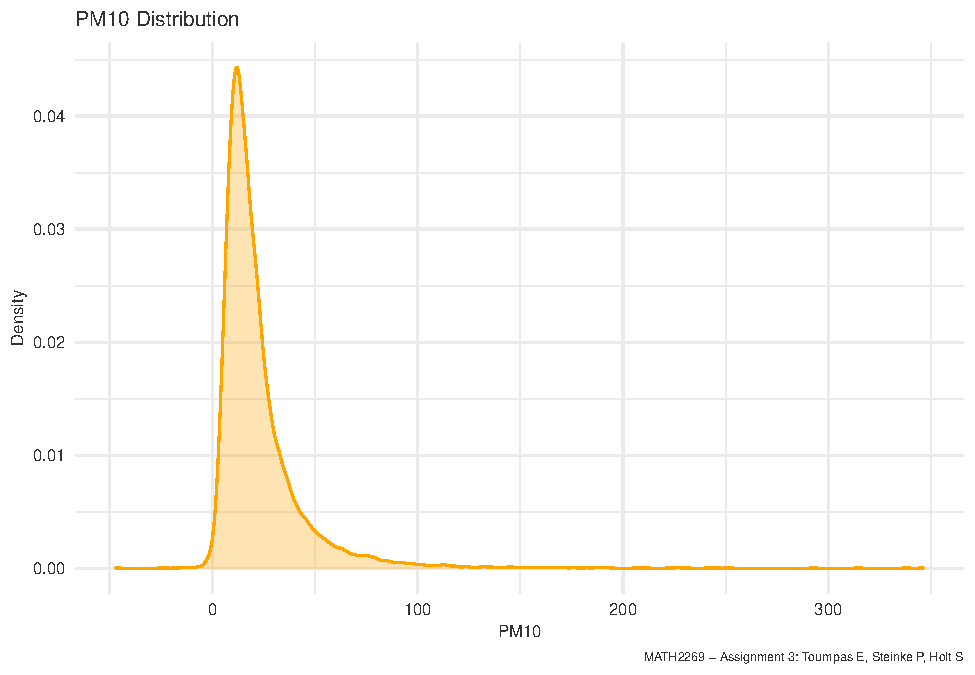
\includegraphics{MATH2269_final_project_files/figure-latex/unnamed-chunk-17-1.pdf}
\caption{PM10 Distribution}
\end{figure}

\hypertarget{correlation-matrix-of-predictors}{%
\paragraph{Correlation matrix of
predictors}\label{correlation-matrix-of-predictors}}

\begin{figure}
\centering
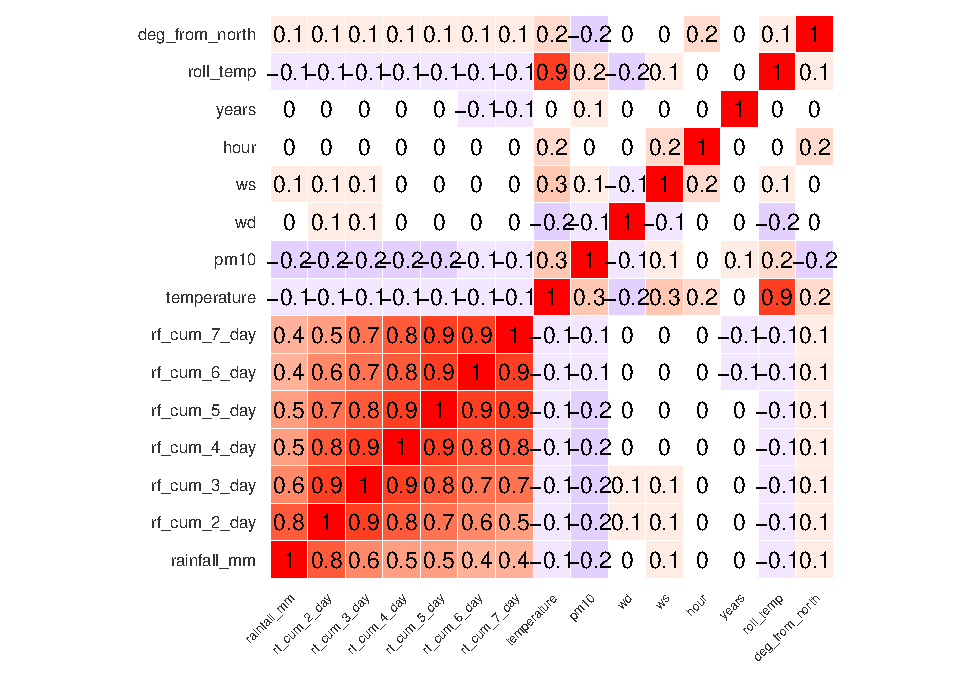
\includegraphics{MATH2269_final_project_files/figure-latex/unnamed-chunk-18-1.pdf}
\caption{Numeric Variable Correlation Heatmap}
\end{figure}

\hypertarget{subsampling}{%
\subsubsection{Subsampling}\label{subsampling}}

\begin{Shaded}
\begin{Highlighting}[]
\CommentTok{# Set temporary values for subsampling trials }
\NormalTok{training_data <-}\StringTok{ }\NormalTok{data_cleaned }\OperatorTok\StringTok{ }
\StringTok{  }\KeywordTok{mutate}\NormalTok{(}\DataTypeTok{pm10 =} \KeywordTok{if_else}\NormalTok{(pm10 }\OperatorTok{<}\StringTok{ }\DecValTok{0}\NormalTok{, }\DecValTok{0}\NormalTok{, pm10)) }\OperatorTok\StringTok{ }
\StringTok{  }\KeywordTok{filter}\NormalTok{(}\OperatorTok{!}\NormalTok{(date_day }\OperatorTok\StringTok{ }\KeywordTok{c}\NormalTok{(}\KeywordTok{ymd}\NormalTok{(}\StringTok{'2018-12-28'}\NormalTok{), }\KeywordTok{ymd}\NormalTok{(}\StringTok{'2018-12-29'}\NormalTok{), }\KeywordTok{ymd}\NormalTok{(}\StringTok{'2018-12-30'}\NormalTok{), }\KeywordTok{ymd}\NormalTok{(}\StringTok{'2018-12-31'}\NormalTok{)))) }\OperatorTok\StringTok{ }
\StringTok{  }\KeywordTok{select}\NormalTok{(}\StringTok{'rf_cum_3_day'}\NormalTok{,}\StringTok{'temperature'}\NormalTok{, }\StringTok{'ws'}\NormalTok{, }\StringTok{'deg_from_north'}\NormalTok{, }\StringTok{'dow'}\NormalTok{, }\StringTok{'working_days'}\NormalTok{, }\StringTok{'hour'}\NormalTok{, }\StringTok{'pre_peak_hour'}\NormalTok{, }\StringTok{'pm10'}\NormalTok{) }\OperatorTok\StringTok{ }
\StringTok{  }\KeywordTok{mutate}\NormalTok{(}\DataTypeTok{dow =} \KeywordTok{as.numeric}\NormalTok{(dow), }
         \DataTypeTok{working_days =} \KeywordTok{as.numeric}\NormalTok{(working_days), }
         \DataTypeTok{pre_peak_hour =} \KeywordTok{as.numeric}\NormalTok{(pre_peak_hour))}

\NormalTok{prediction_data <-}\StringTok{ }\NormalTok{data_cleaned }\OperatorTok\StringTok{ }
\StringTok{  }\KeywordTok{mutate}\NormalTok{(}\DataTypeTok{pm10 =} \KeywordTok{if_else}\NormalTok{(pm10 }\OperatorTok{<}\StringTok{ }\DecValTok{0}\NormalTok{, }\DecValTok{0}\NormalTok{, pm10)) }\OperatorTok\StringTok{ }
\StringTok{  }\KeywordTok{filter}\NormalTok{(date_day }\OperatorTok\StringTok{ }\KeywordTok{c}\NormalTok{(}\KeywordTok{ymd}\NormalTok{(}\StringTok{'2018-12-28'}\NormalTok{), }\KeywordTok{ymd}\NormalTok{(}\StringTok{'2018-12-29'}\NormalTok{), }\KeywordTok{ymd}\NormalTok{(}\StringTok{'2018-12-30'}\NormalTok{), }\KeywordTok{ymd}\NormalTok{(}\StringTok{'2018-12-31'}\NormalTok{))) }\OperatorTok\StringTok{ }
\StringTok{  }\KeywordTok{select}\NormalTok{(}\StringTok{'rf_cum_3_day'}\NormalTok{,}\StringTok{'temperature'}\NormalTok{, }\StringTok{'ws'}\NormalTok{, }\StringTok{'deg_from_north'}\NormalTok{, }\StringTok{'dow'}\NormalTok{, }\StringTok{'working_days'}\NormalTok{, }\StringTok{'hour'}\NormalTok{, }\StringTok{'pre_peak_hour'}\NormalTok{)   }\OperatorTok\StringTok{ }
\StringTok{  }\KeywordTok{mutate}\NormalTok{(}\DataTypeTok{dow =} \KeywordTok{as.numeric}\NormalTok{(dow), }
         \DataTypeTok{working_days =} \KeywordTok{as.numeric}\NormalTok{(working_days), }
         \DataTypeTok{pre_peak_hour =} \KeywordTok{as.numeric}\NormalTok{(pre_peak_hour))}

\CommentTok{# Mean specification}
\NormalTok{mu <-}\StringTok{ }\KeywordTok{c}\NormalTok{(}\OperatorTok{-}\DecValTok{40}\NormalTok{, }\DecValTok{40}\NormalTok{, }\DecValTok{0}\NormalTok{, }\DecValTok{-40}\NormalTok{, }\DecValTok{0}\NormalTok{, }\DecValTok{20}\NormalTok{, }\DecValTok{0}\NormalTok{, }\DecValTok{20}\NormalTok{)}

\CommentTok{# Variance specification}
\NormalTok{var  <-}\StringTok{ }\KeywordTok{c}\NormalTok{(}\DecValTok{1}\OperatorTok{/}\DecValTok{4}\NormalTok{,}\DecValTok{1}\OperatorTok{/}\DecValTok{2}\NormalTok{,}\DecValTok{1}\OperatorTok{/}\DecValTok{10}\NormalTok{,}\DecValTok{1}\OperatorTok{/}\DecValTok{2}\NormalTok{,}\DecValTok{1}\OperatorTok{/}\DecValTok{10}\NormalTok{,}\DecValTok{1}\OperatorTok{/}\DecValTok{2}\NormalTok{,}\DecValTok{1}\OperatorTok{/}\DecValTok{10}\NormalTok{,}\DecValTok{1}\OperatorTok{/}\DecValTok{2}\NormalTok{)}

\CommentTok{# Parameters to use}
\NormalTok{use_parameters <-}\StringTok{ }\KeywordTok{list}\NormalTok{(}\DataTypeTok{number_chains =} \DecValTok{3}\NormalTok{, }\DataTypeTok{number_adaptation_steps =} \DecValTok{200}\NormalTok{, }\DataTypeTok{burn_in_steps =} \DecValTok{200}\NormalTok{, }\DataTypeTok{thinning_steps =} \DecValTok{3}\NormalTok{)}
\end{Highlighting}
\end{Shaded}

\begin{Shaded}
\begin{Highlighting}[]
\CommentTok{# Select variables}
\NormalTok{predictor_variable <-}\StringTok{ 'pm10'}

\CommentTok{# Set up prediction values}
\NormalTok{xPred =}\StringTok{ }\KeywordTok{array}\NormalTok{(}\OtherTok{NA}\NormalTok{, }\DataTypeTok{dim =} \KeywordTok{c}\NormalTok{(}\KeywordTok{nrow}\NormalTok{(prediction_data), }\KeywordTok{length}\NormalTok{(}\KeywordTok{colnames}\NormalTok{(prediction_data))))}

\ControlFlowTok{for}\NormalTok{(i }\ControlFlowTok{in} \DecValTok{1}\OperatorTok{:}\KeywordTok{nrow}\NormalTok{(prediction_data))\{}
\NormalTok{  xPred[i,] =}\StringTok{ }\KeywordTok{c}\NormalTok{(prediction_data[[i,}\DecValTok{1}\NormalTok{]], }
\NormalTok{                prediction_data[[i,}\DecValTok{2}\NormalTok{]], }
\NormalTok{                prediction_data[[i,}\DecValTok{3}\NormalTok{]], }
\NormalTok{                prediction_data[[i,}\DecValTok{4}\NormalTok{]], }
\NormalTok{                prediction_data[[i,}\DecValTok{5}\NormalTok{]], }
\NormalTok{                prediction_data[[i,}\DecValTok{6}\NormalTok{]], }
\NormalTok{                prediction_data[[i,}\DecValTok{7}\NormalTok{]], }
\NormalTok{                prediction_data[[i,}\DecValTok{8}\NormalTok{]])}
\NormalTok{\}}
\end{Highlighting}
\end{Shaded}

\hypertarget{subsample-size-trials}{%
\paragraph{Subsample size trials}\label{subsample-size-trials}}

\begin{Shaded}
\begin{Highlighting}[]
\NormalTok{trial_type <-}\StringTok{ "subsample_size"}

\ControlFlowTok{if}\NormalTok{(}\KeywordTok{hasnt_run}\NormalTok{(trial_type))\{}

  \CommentTok{# Set seeds}
\NormalTok{  seed_value <-}\StringTok{ }\KeywordTok{sample}\NormalTok{(}\DecValTok{1}\OperatorTok{:}\DecValTok{10000}\NormalTok{, }\DecValTok{20}\NormalTok{, }\DataTypeTok{replace=}\NormalTok{F)}
  \KeywordTok{write.csv}\NormalTok{(seed_value, }\KeywordTok{paste0}\NormalTok{(}\KeywordTok{here}\NormalTok{(),}\StringTok{"/OUTPUTS/SEEDS/"}\NormalTok{,trial_type,}\StringTok{"_seeds.csv"}\NormalTok{), }\DataTypeTok{row.names =} \OtherTok{FALSE}\NormalTok{)}
  
  \CommentTok{# Set up sample size trial values}
\NormalTok{  sample_size_list <-}\StringTok{ }\KeywordTok{c}\NormalTok{(}\DecValTok{100}\NormalTok{, }\DecValTok{500}\NormalTok{, }\DecValTok{1000}\NormalTok{, }\DecValTok{2000}\NormalTok{, }\DecValTok{2500}\NormalTok{, }\DecValTok{5000}\NormalTok{)}
  
  \CommentTok{# Set up trial df and set up columns}
\NormalTok{  subsample_size_trials <-}\StringTok{ }\KeywordTok{expand.grid}\NormalTok{(}\DataTypeTok{sampling_size =}\NormalTok{ sample_size_list, }\DataTypeTok{seed =}\NormalTok{ seed_value)}
\NormalTok{  subsample_size_trials[}\KeywordTok{c}\NormalTok{(}\KeywordTok{paste0}\NormalTok{(}\KeywordTok{colnames}\NormalTok{(training_data),}\StringTok{"_p_value"}\NormalTok{), }\StringTok{"duration"}\NormalTok{)] <-}\StringTok{ }\DecValTok{0}
\NormalTok{  subsample_size_trials[}\StringTok{'trial_number'}\NormalTok{] <-}\StringTok{ }\DecValTok{1}\OperatorTok{:}\KeywordTok{nrow}\NormalTok{(subsample_size_trials)}

  \CommentTok{# Added more trials later}
\NormalTok{  sample_size_list_more <-}\StringTok{ }\KeywordTok{c}\NormalTok{(}\DecValTok{7500}\NormalTok{, }\DecValTok{10000}\NormalTok{)}
\NormalTok{  subsample_size_trials_more <-}\StringTok{ }\KeywordTok{expand.grid}\NormalTok{(}\DataTypeTok{sampling_size =}\NormalTok{ sample_size_list_more, }\DataTypeTok{seed =}\NormalTok{ seed_value)}
\NormalTok{  subsample_size_trials_more[}\KeywordTok{c}\NormalTok{(}\KeywordTok{paste0}\NormalTok{(}\KeywordTok{colnames}\NormalTok{(training_data),}\StringTok{"_p_value"}\NormalTok{), }\StringTok{"duration"}\NormalTok{)] <-}\StringTok{ }\DecValTok{0}
\NormalTok{  subsample_size_trials_more[}\StringTok{'trial_number'}\NormalTok{] <-}\StringTok{ }\NormalTok{(}\DecValTok{1}\OperatorTok{+}\KeywordTok{nrow}\NormalTok{(subsample_size_trials))}\OperatorTok{:}\NormalTok{(}\KeywordTok{nrow}\NormalTok{(subsample_size_trials_more)}\OperatorTok{+}\KeywordTok{nrow}\NormalTok{(subsample_size_trials))}
\NormalTok{  old_n <-}\StringTok{ }\KeywordTok{nrow}\NormalTok{(subsample_size_trials)}
\NormalTok{  subsample_size_trials <-}\StringTok{ }\KeywordTok{rbind}\NormalTok{(subsample_size_trials,subsample_size_trials_more)}
  
  
  \CommentTok{# Run Subsampling trials}
  \ControlFlowTok{for}\NormalTok{(row }\ControlFlowTok{in} \DecValTok{1}\OperatorTok{:}\KeywordTok{nrow}\NormalTok{(subsample_size_trials))\{}
    
    \KeywordTok{print}\NormalTok{(}\KeywordTok{paste0}\NormalTok{(}\StringTok{'Running trial '}\NormalTok{,row))}
    
    \CommentTok{# Running subsample size trial}
\NormalTok{    returned_values <-}\StringTok{ }\KeywordTok{run_subsample_trial}\NormalTok{(}\DataTypeTok{trial_df =}\NormalTok{ subsample_size_trials, }\DataTypeTok{row_num =}\NormalTok{ row, }
                                                              \DataTypeTok{full_sample =}\NormalTok{ training_data, }\DataTypeTok{trial_name =} \StringTok{'subsampling_size'}\NormalTok{)}
    
\NormalTok{    returned_candidate_sample_selected <-}\StringTok{ }\NormalTok{returned_values}\OperatorTok{$}\NormalTok{candidate_sample_selected}
\NormalTok{    subsample_size_trials <-}\StringTok{ }\NormalTok{returned_values}\OperatorTok{$}\NormalTok{trial_df}
    \KeywordTok{print}\NormalTok{(}\StringTok{'Candidate sample selected'}\NormalTok{)}
    
    \CommentTok{# Deal with 0 pm10 levels}
\NormalTok{    returned_candidate_sample_selected}\OperatorTok{$}\NormalTok{pm10 <-}\StringTok{ }\NormalTok{returned_candidate_sample_selected}\OperatorTok{$}\NormalTok{pm10 }\OperatorTok{+}\StringTok{ }\FloatTok{0.1} 
    
    \CommentTok{# Select initial values based on candidate subsample}
\NormalTok{    sd_rf_cum_}\DecValTok{3}\NormalTok{_day <-}\StringTok{   }\KeywordTok{sd}\NormalTok{(returned_candidate_sample_selected}\OperatorTok{$}\NormalTok{rf_cum_}\DecValTok{3}\NormalTok{_day)}
\NormalTok{    sd_temperature <-}\StringTok{   }\KeywordTok{sd}\NormalTok{(returned_candidate_sample_selected}\OperatorTok{$}\NormalTok{temperature)}
\NormalTok{    sd_ws <-}\StringTok{   }\KeywordTok{sd}\NormalTok{(returned_candidate_sample_selected}\OperatorTok{$}\NormalTok{ws)}
\NormalTok{    sd_deg_from_north <-}\StringTok{   }\KeywordTok{sd}\NormalTok{(returned_candidate_sample_selected}\OperatorTok{$}\NormalTok{deg_from_north)}
\NormalTok{    sd_dow <-}\StringTok{   }\KeywordTok{sd}\NormalTok{(returned_candidate_sample_selected}\OperatorTok{$}\NormalTok{dow)}
\NormalTok{    sd_working_days <-}\StringTok{   }\KeywordTok{sd}\NormalTok{(returned_candidate_sample_selected}\OperatorTok{$}\NormalTok{working_days)}
\NormalTok{    sd_hour <-}\StringTok{   }\KeywordTok{sd}\NormalTok{(returned_candidate_sample_selected}\OperatorTok{$}\NormalTok{hour)}
\NormalTok{    sd_pre_peak_hour <-}\StringTok{   }\KeywordTok{sd}\NormalTok{(returned_candidate_sample_selected}\OperatorTok{$}\NormalTok{pre_peak_hour)}
\NormalTok{    sd_pm10 <-}\StringTok{   }\KeywordTok{sd}\NormalTok{(returned_candidate_sample_selected}\OperatorTok{$}\NormalTok{pm10)}
    
\NormalTok{    initial_values_list <-}\StringTok{ }\KeywordTok{c}\NormalTok{(}\FloatTok{0.1}\NormalTok{,}
                             \KeywordTok{mean}\NormalTok{(returned_candidate_sample_selected}\OperatorTok{$}\NormalTok{rf_cum_}\DecValTok{3}\NormalTok{_day)}\OperatorTok{/}\NormalTok{sd_rf_cum_}\DecValTok{3}\NormalTok{_day, }
                             \KeywordTok{mean}\NormalTok{(returned_candidate_sample_selected}\OperatorTok{$}\NormalTok{temperature)}\OperatorTok{/}\NormalTok{sd_temperature, }
                             \KeywordTok{mean}\NormalTok{(returned_candidate_sample_selected}\OperatorTok{$}\NormalTok{ws)}\OperatorTok{/}\NormalTok{sd_ws, }
                             \KeywordTok{mean}\NormalTok{(returned_candidate_sample_selected}\OperatorTok{$}\NormalTok{deg_from_north)}\OperatorTok{/}\NormalTok{sd_deg_from_north, }
                             \KeywordTok{mean}\NormalTok{(returned_candidate_sample_selected}\OperatorTok{$}\NormalTok{dow)}\OperatorTok{/}\NormalTok{sd_dow, }
                             \KeywordTok{mean}\NormalTok{(returned_candidate_sample_selected}\OperatorTok{$}\NormalTok{working_days)}\OperatorTok{/}\NormalTok{sd_working_days, }
                             \KeywordTok{mean}\NormalTok{(returned_candidate_sample_selected}\OperatorTok{$}\NormalTok{hour)}\OperatorTok{/}\NormalTok{sd_hour,}
                             \KeywordTok{mean}\NormalTok{(returned_candidate_sample_selected}\OperatorTok{$}\NormalTok{pre_peak_hour)}\OperatorTok{/}\NormalTok{sd_pre_peak_hour,}
                             \FloatTok{0.01}\NormalTok{)}

    \CommentTok{# Run JAGS model with candidate sample}
\NormalTok{    returned_values <-}\StringTok{ }\KeywordTok{run_subsample_size_JAGS_trial}\NormalTok{(}\DataTypeTok{data =}\NormalTok{ returned_candidate_sample_selected, }
                                                     \DataTypeTok{predictor =} \StringTok{"pm10"}\NormalTok{, }
                                                     \DataTypeTok{predictions =}\NormalTok{ xPred, }
                                                     \DataTypeTok{mu_list =}\NormalTok{ mu, }
                                                     \DataTypeTok{var_list =}\NormalTok{ var,}
                                                     \DataTypeTok{initial_values =}\NormalTok{ initial_values_list, }
                                                     \DataTypeTok{params =}\NormalTok{ use_parameters, }
                                                     \DataTypeTok{trial_num =}\NormalTok{ row)}
    \KeywordTok{print}\NormalTok{(}\StringTok{'JAGS model run'}\NormalTok{)}
    
    \CommentTok{# Save time elapsed for the model - Store}
\NormalTok{    subsample_size_trials[row, }\StringTok{"duration"}\NormalTok{] <-}\StringTok{ }\NormalTok{returned_values[}\StringTok{'time_elapsed'}\NormalTok{]}
    \KeywordTok{write.csv}\NormalTok{(subsample_size_trials, }\KeywordTok{paste0}\NormalTok{(}\KeywordTok{here}\NormalTok{(),}\StringTok{'/OUTPUTS/TRIAL_INFO/'}\NormalTok{,trial_type,}\StringTok{'_trials.csv'}\NormalTok{), }\DataTypeTok{row.names =} \OtherTok{FALSE}\NormalTok{)}
  
    \CommentTok{# Save RData }
    \KeywordTok{save.image}\NormalTok{(}\DataTypeTok{file =} \StringTok{"subsample_size_trials.RData"}\NormalTok{)}
    
    \CommentTok{# Reset}
    \KeywordTok{graphics.off}\NormalTok{()}
    
\NormalTok{  \}}
  
\NormalTok{  subsample_size_trials <-}\StringTok{ }\NormalTok{subsample_size_trials }\OperatorTok\StringTok{ }
\StringTok{    }\KeywordTok{mutate}\NormalTok{(}\DataTypeTok{mean_p_value =} \KeywordTok{rowMeans}\NormalTok{(subsample_size_trials[}\KeywordTok{c}\NormalTok{(}\StringTok{'rf_cum_3_day_p_value'}\NormalTok{, }\StringTok{'temperature_p_value'}\NormalTok{, }\StringTok{'ws_p_value'}\NormalTok{, }\StringTok{'deg_from_north_p_value'}\NormalTok{, }\StringTok{'dow_p_value'}\NormalTok{, }
                                                           \StringTok{'working_days_p_value'}\NormalTok{, }\StringTok{'hour_p_value'}\NormalTok{, }\StringTok{'pre_peak_hour_p_value'}\NormalTok{, }\StringTok{'pm10_p_value'}\NormalTok{)]))}
   
  \KeywordTok{write.csv}\NormalTok{(subsample_size_trials, }\KeywordTok{paste0}\NormalTok{(}\KeywordTok{here}\NormalTok{(),}\StringTok{'/OUTPUTS/TRIAL_INFO/'}\NormalTok{,trial_type,}\StringTok{'_trials.csv'}\NormalTok{), }\DataTypeTok{row.names =} \OtherTok{FALSE}\NormalTok{)}

\NormalTok{\} }\ControlFlowTok{else}\NormalTok{ \{}
  
  \KeywordTok{print}\NormalTok{(}\StringTok{'Already run'}\NormalTok{)}
  
\NormalTok{\}}
\end{Highlighting}
\end{Shaded}

\begin{verbatim}
## [1] "Already run"
\end{verbatim}

\begin{Shaded}
\begin{Highlighting}[]
\NormalTok{subsample_size_trials <-}\StringTok{ }\KeywordTok{read.csv}\NormalTok{(}\KeywordTok{paste0}\NormalTok{(}\KeywordTok{here}\NormalTok{(),}\StringTok{'/OUTPUTS/TRIAL_INFO/'}\NormalTok{,trial_type,}\StringTok{'_trials.csv'}\NormalTok{), }\DataTypeTok{stringsAsFactors =} \OtherTok{FALSE}\NormalTok{) }\OperatorTok\StringTok{ }
\StringTok{  }\KeywordTok{arrange}\NormalTok{(trial_number)}

\NormalTok{sample_data <-}\StringTok{ }\NormalTok{subsample_size_trials }\OperatorTok\StringTok{ }
\StringTok{  }\KeywordTok{select}\NormalTok{(}\KeywordTok{c}\NormalTok{(trial_number, sampling_size, duration, mean_p_value)) }\OperatorTok\StringTok{ }
\StringTok{  }\KeywordTok{arrange}\NormalTok{(trial_number) }\OperatorTok\StringTok{ }
\StringTok{  }\KeywordTok{mutate}\NormalTok{(}\DataTypeTok{sampling_size =} \KeywordTok{factor}\NormalTok{(sampling_size, }\DataTypeTok{levels =} \KeywordTok{c}\NormalTok{(}\StringTok{'100'}\NormalTok{, }\StringTok{'500'}\NormalTok{, }\StringTok{'1000'}\NormalTok{, }\StringTok{'2000'}\NormalTok{, }\StringTok{'2500'}\NormalTok{, }\StringTok{'5000'}\NormalTok{, }\StringTok{'7500'}\NormalTok{, }\StringTok{'10000'}\NormalTok{))) }

\NormalTok{sample_data  }\OperatorTok\StringTok{ }
\StringTok{  }\KeywordTok{head}\NormalTok{(}\DecValTok{25}\NormalTok{) }\OperatorTok\StringTok{ }
\StringTok{  }\KeywordTok{format_table}\NormalTok{(}\DataTypeTok{p_caption =} \StringTok{"First 25 records of the results from the subsample size trials"}\NormalTok{)}
\end{Highlighting}
\end{Shaded}

\begin{table}

\caption{\label{tab:unnamed-chunk-21}First 25 records of the results from the subsample size trials}
\centering
\begin{tabu} to \linewidth {>{\raggedleft}X>{\raggedright}X>{\raggedleft}X>{\raggedleft}X}
\hline
trial\_number & sampling\_size & duration & mean\_p\_value\\
\hline
1 & 100 & 29.10087 & 0.7150044\\
\hline
2 & 500 & 46.92803 & 0.8020683\\
\hline
3 & 1000 & 72.11060 & 0.6437267\\
\hline
4 & 2000 & 127.93469 & 0.7826845\\
\hline
5 & 2500 & 156.81991 & 0.7391136\\
\hline
6 & 5000 & 310.13877 & 0.7390285\\
\hline
7 & 100 & 27.91725 & 0.5694091\\
\hline
8 & 500 & 44.28588 & 0.7923011\\
\hline
9 & 1000 & 71.85435 & 0.6376434\\
\hline
10 & 2000 & 128.59651 & 0.6409041\\
\hline
11 & 2500 & 153.68574 & 0.7451210\\
\hline
12 & 5000 & 294.93467 & 0.8292943\\
\hline
13 & 100 & 32.26039 & 0.6291223\\
\hline
14 & 500 & 47.82899 & 0.7336884\\
\hline
15 & 1000 & 83.59841 & 0.4722391\\
\hline
16 & 2000 & 134.04626 & 0.6401590\\
\hline
17 & 2500 & 164.22629 & 0.6231998\\
\hline
18 & 5000 & 298.02577 & 0.9581253\\
\hline
19 & 100 & 29.56241 & 0.7608085\\
\hline
20 & 500 & 44.74994 & 0.7202849\\
\hline
21 & 1000 & 69.82387 & 0.7799489\\
\hline
22 & 2000 & 140.67582 & 0.7412632\\
\hline
23 & 2500 & 165.72553 & 0.8085898\\
\hline
24 & 5000 & 319.81962 & 0.7315819\\
\hline
25 & 100 & 28.52830 & 0.5227476\\
\hline
\end{tabu}
\end{table}

\begin{figure}
\centering
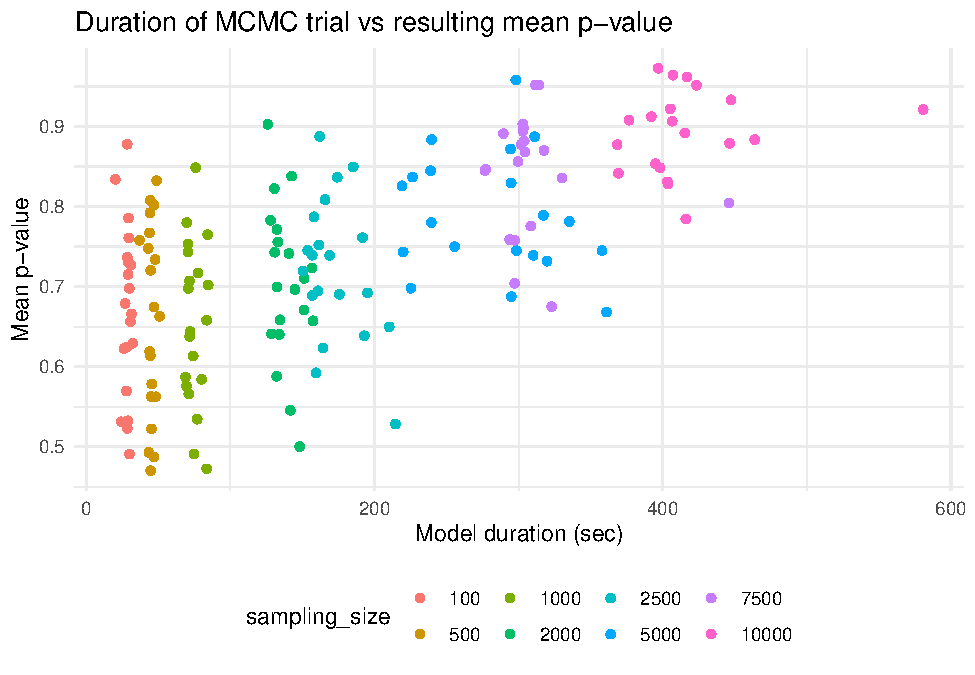
\includegraphics{MATH2269_final_project_files/figure-latex/unnamed-chunk-22-1.pdf}
\caption{Scatter plot of all trials}
\end{figure}

\begin{Shaded}
\begin{Highlighting}[]
\NormalTok{sample_data }\OperatorTok\StringTok{ }
\StringTok{  }\KeywordTok{group_by}\NormalTok{(sampling_size) }\OperatorTok\StringTok{ }
\StringTok{  }\KeywordTok{summarise}\NormalTok{(}\DataTypeTok{mean_p_value =} \KeywordTok{mean}\NormalTok{(mean_p_value), }
            \DataTypeTok{mean_duration =} \KeywordTok{mean}\NormalTok{(duration)) }\OperatorTok\StringTok{ }
\StringTok{  }\KeywordTok{format_table}\NormalTok{(}\DataTypeTok{p_caption =} \StringTok{"Full set of results from the subsample size trials"}\NormalTok{)}
\end{Highlighting}
\end{Shaded}

\begin{verbatim}
## `summarise()` ungrouping output (override with `.groups` argument)
\end{verbatim}

\begin{table}

\caption{\label{tab:unnamed-chunk-23}Full set of results from the subsample size trials}
\centering
\begin{tabu} to \linewidth {>{\raggedright}X>{\raggedleft}X>{\raggedleft}X}
\hline
sampling\_size & mean\_p\_value & mean\_duration\\
\hline
100 & 0.6694404 & 28.57028\\
\hline
500 & 0.6602828 & 45.35113\\
\hline
1000 & 0.6537587 & 75.16514\\
\hline
2000 & 0.7043481 & 138.81699\\
\hline
2500 & 0.7211568 & 172.92682\\
\hline
5000 & 0.7897317 & 282.90547\\
\hline
7500 & 0.8423146 & 310.10076\\
\hline
10000 & 0.8935942 & 416.61689\\
\hline
\end{tabu}
\end{table}

\hypertarget{subsample-selection-trials}{%
\paragraph{Subsample selection
trials}\label{subsample-selection-trials}}

\begin{Shaded}
\begin{Highlighting}[]
\NormalTok{trial_type <-}\StringTok{ "subsample_selection"}

\ControlFlowTok{if}\NormalTok{(}\KeywordTok{hasnt_run}\NormalTok{(trial_type))\{}

  \CommentTok{# Set seeds}
\NormalTok{  seed_value <-}\StringTok{ }\KeywordTok{sample}\NormalTok{(}\DecValTok{1}\OperatorTok{:}\DecValTok{10000}\NormalTok{, }\DecValTok{100}\NormalTok{, }\DataTypeTok{replace=}\NormalTok{F)}
  \KeywordTok{write.csv}\NormalTok{(seed_value, }\KeywordTok{paste0}\NormalTok{(}\KeywordTok{here}\NormalTok{(),}\StringTok{"/OUTPUTS/SEEDS/"}\NormalTok{,trial_type,}\StringTok{"_seeds.csv"}\NormalTok{), }\DataTypeTok{row.names =} \OtherTok{FALSE}\NormalTok{)}
  
  \CommentTok{# Set up sample size trial values}
\NormalTok{  sample_size_list <-}\StringTok{ }\KeywordTok{c}\NormalTok{(}\DecValTok{1000}\NormalTok{)}
  
  \CommentTok{# Set up trial df and set up columns}
\NormalTok{  subsample_selection_trials <-}\StringTok{ }\KeywordTok{expand.grid}\NormalTok{(}\DataTypeTok{sampling_size =}\NormalTok{ sample_size_list, }\DataTypeTok{seed =}\NormalTok{ seed_value)}
\NormalTok{  subsample_selection_trials[}\KeywordTok{c}\NormalTok{(}\KeywordTok{paste0}\NormalTok{(}\KeywordTok{colnames}\NormalTok{(training_data),}\StringTok{"_p_value"}\NormalTok{), }\StringTok{"duration"}\NormalTok{)] <-}\StringTok{ }\DecValTok{0}
\NormalTok{  subsample_selection_trials[}\StringTok{'trial_number'}\NormalTok{] <-}\StringTok{ }\DecValTok{1}\OperatorTok{:}\KeywordTok{nrow}\NormalTok{(subsample_selection_trials)}
  
  \CommentTok{# Run Subsampling trials}
  \ControlFlowTok{for}\NormalTok{(row }\ControlFlowTok{in} \DecValTok{1}\OperatorTok{:}\KeywordTok{nrow}\NormalTok{(subsample_selection_trials))\{}
    
    \KeywordTok{print}\NormalTok{(}\KeywordTok{paste0}\NormalTok{(}\StringTok{'Running trial '}\NormalTok{,row))}
    
    \CommentTok{# Running subsample size trial}
\NormalTok{    returned_values <-}\StringTok{ }\KeywordTok{run_subsample_trial}\NormalTok{(}\DataTypeTok{trial_df =}\NormalTok{ subsample_selection_trials, }\DataTypeTok{row_num =}\NormalTok{ row, }
                                                              \DataTypeTok{full_sample =}\NormalTok{ training_data, }\DataTypeTok{trial_name =}\NormalTok{ trial_type)}
\NormalTok{    subsample_selection_trials <-}\StringTok{ }\NormalTok{returned_values}\OperatorTok{$}\NormalTok{trial_df}

    \CommentTok{# Save time elapsed for the model - Store}
    \KeywordTok{write.csv}\NormalTok{(subsample_selection_trials, }\KeywordTok{paste0}\NormalTok{(}\KeywordTok{here}\NormalTok{(),}\StringTok{'/OUTPUTS/TRIAL_INFO/'}\NormalTok{,trial_type,}\StringTok{'_trials.csv'}\NormalTok{), }\DataTypeTok{row.names =} \OtherTok{FALSE}\NormalTok{)}
  
    \CommentTok{# Save RData }
    \KeywordTok{save.image}\NormalTok{(}\DataTypeTok{file =} \StringTok{"subsample_selection_trials.RData"}\NormalTok{)}
\NormalTok{  \}}
  
  
  \CommentTok{# When selecting all candidate subsamples, a mean p-value for each trial is calculated}
\NormalTok{   subsample_selection_trials <-}\StringTok{ }\NormalTok{subsample_selection_trials }\OperatorTok\StringTok{ }
\StringTok{    }\KeywordTok{mutate}\NormalTok{(}\DataTypeTok{mean_p_value =} \KeywordTok{rowMeans}\NormalTok{(subsample_selection_trials[}\KeywordTok{c}\NormalTok{(}\StringTok{'rf_cum_3_day_p_value'}\NormalTok{, }\StringTok{'temperature_p_value'}\NormalTok{, }\StringTok{'ws_p_value'}\NormalTok{, }
                                                                \StringTok{'deg_from_north_p_value'}\NormalTok{, }\StringTok{'dow_p_value'}\NormalTok{, }\StringTok{'working_days_p_value'}\NormalTok{, }
                                                                \StringTok{'hour_p_value'}\NormalTok{, }\StringTok{'pre_peak_hour_p_value'}\NormalTok{, }\StringTok{'pm10_p_value'}\NormalTok{)]))}
   
   \CommentTok{# These results are saved}
  \KeywordTok{write.csv}\NormalTok{(subsample_selection_trials, }\KeywordTok{paste0}\NormalTok{(}\KeywordTok{here}\NormalTok{(),}\StringTok{'/OUTPUTS/TRIAL_INFO/'}\NormalTok{,trial_type,}\StringTok{'_trials.csv'}\NormalTok{), }\DataTypeTok{row.names =} \OtherTok{FALSE}\NormalTok{)}
  

\NormalTok{\} }\ControlFlowTok{else}\NormalTok{ \{}
  
  \KeywordTok{print}\NormalTok{(}\StringTok{'Already run'}\NormalTok{)}
  
\NormalTok{\}}
\end{Highlighting}
\end{Shaded}

\begin{verbatim}
## [1] "Already run"
\end{verbatim}

\begin{Shaded}
\begin{Highlighting}[]
\NormalTok{subsample_selection_trials <-}\StringTok{ }\KeywordTok{read.csv}\NormalTok{(}\KeywordTok{paste0}\NormalTok{(}\KeywordTok{here}\NormalTok{(),}\StringTok{'/OUTPUTS/TRIAL_INFO/'}\NormalTok{,trial_type,}\StringTok{'_trials.csv'}\NormalTok{), }\DataTypeTok{stringsAsFactors =} \OtherTok{FALSE}\NormalTok{) }\OperatorTok\StringTok{ }
\StringTok{  }\KeywordTok{select}\NormalTok{(}\StringTok{'trial_number'}\NormalTok{, }\StringTok{'mean_p_value'}\NormalTok{,}\StringTok{'rf_cum_3_day_p_value'}\NormalTok{, }\StringTok{'temperature_p_value'}\NormalTok{, }\StringTok{'ws_p_value'}\NormalTok{, }\StringTok{'deg_from_north_p_value'}\NormalTok{, }
         \StringTok{'dow_p_value'}\NormalTok{, }\StringTok{'working_days_p_value'}\NormalTok{, }\StringTok{'hour_p_value'}\NormalTok{, }\StringTok{'pre_peak_hour_p_value'}\NormalTok{, }\StringTok{'pm10_p_value'}\NormalTok{)}

\NormalTok{subsample_selection_trials }\OperatorTok\StringTok{ }
\StringTok{  }\KeywordTok{arrange}\NormalTok{(}\KeywordTok{desc}\NormalTok{(mean_p_value)) }\OperatorTok\StringTok{ }
\StringTok{  `}\DataTypeTok{colnames<-}\StringTok{`}\NormalTok{(}\KeywordTok{gsub}\NormalTok{(}\StringTok{"_"}\NormalTok{, }\StringTok{" "}\NormalTok{,}\KeywordTok{colnames}\NormalTok{(subsample_selection_trials))) }\OperatorTok\StringTok{ }
\StringTok{  }\KeywordTok{head}\NormalTok{(}\DecValTok{5}\NormalTok{) }\OperatorTok\StringTok{ }
\StringTok{  }\KeywordTok{format_table}\NormalTok{(}\DataTypeTok{p_caption =} \StringTok{"The top five candidate subselections in the subsample selection trials."}\NormalTok{, }\DataTypeTok{width =} \OtherTok{TRUE}\NormalTok{) }
\end{Highlighting}
\end{Shaded}

\begin{table}

\caption{\label{tab:unnamed-chunk-25}The top five candidate subselections in the subsample selection trials.}
\centering
\begin{tabu} to \linewidth {>{\raggedleft}X>{\raggedleft}X>{\raggedleft}X>{\raggedleft}X>{\raggedleft}X>{\raggedleft}X>{\raggedleft}X>{\raggedleft}X>{\raggedleft}X>{\raggedleft}X>{\raggedleft}X}
\hline
trial number & mean p value & rf cum 3 day p value & temperature p value & ws p value & deg from north p value & dow p value & working days p value & hour p value & pre peak hour p value & pm10 p value\\
\hline
7 & 0.9335038 & 0.9179127 & 0.8800272 & 0.8615146 & 0.9527719 & 1.0000000 & 1.0000000 & 0.8015225 & 0.9999915 & 0.9877941\\
\hline
92 & 0.8844267 & 0.9929617 & 0.9518290 & 0.6624545 & 0.9220733 & 0.9809347 & 0.9809347 & 0.6664733 & 1.0000000 & 0.8021792\\
\hline
59 & 0.8826383 & 0.9994628 & 0.9669227 & 0.9448022 & 0.8660622 & 0.9999993 & 1.0000000 & 0.8545957 & 0.9588906 & 0.3530091\\
\hline
75 & 0.8530036 & 0.9697510 & 0.9118581 & 0.6231489 & 0.9406564 & 0.8810719 & 0.8810719 & 0.9058613 & 1.0000000 & 0.5636127\\
\hline
62 & 0.8453595 & 0.9969976 & 0.1919882 & 0.9935657 & 0.9804068 & 0.9999981 & 1.0000000 & 0.7198917 & 0.9726895 & 0.7526976\\
\hline
\end{tabu}
\end{table}

\begin{Shaded}
\begin{Highlighting}[]
\NormalTok{subsampled_data <-}\StringTok{ }\KeywordTok{read.csv}\NormalTok{(}\KeywordTok{paste0}\NormalTok{(}\KeywordTok{here}\NormalTok{(),}\StringTok{'/OUTPUTS/SAMPLES/SUBSAMPLE_SELECTION_TRIAL/subsample_selection_trial_candidate_subsample_7.csv'}\NormalTok{))}

\NormalTok{subsampled_data}\OperatorTok{$}\NormalTok{pm10 <-}\StringTok{ }\NormalTok{subsampled_data}\OperatorTok{$}\NormalTok{pm10 }\OperatorTok{+}\StringTok{ }\FloatTok{0.01}
\end{Highlighting}
\end{Shaded}

\hypertarget{mathematical-model}{%
\subsubsection{Mathematical model}\label{mathematical-model}}

\hypertarget{prior-specification}{%
\subsubsection{Prior specification}\label{prior-specification}}

\hypertarget{model}{%
\subsubsection{Model}\label{model}}

\begin{Shaded}
\begin{Highlighting}[]
\CommentTok{# Mean specification}
\NormalTok{mu <-}\StringTok{ }\KeywordTok{c}\NormalTok{(}\OperatorTok{-}\DecValTok{40}\NormalTok{, }\DecValTok{40}\NormalTok{, }\DecValTok{0}\NormalTok{, }\DecValTok{-40}\NormalTok{, }\DecValTok{0}\NormalTok{, }\DecValTok{20}\NormalTok{, }\DecValTok{0}\NormalTok{, }\DecValTok{20}\NormalTok{)}

\CommentTok{# Variance specification}
\NormalTok{var  <-}\StringTok{ }\KeywordTok{c}\NormalTok{(}\DecValTok{1}\OperatorTok{/}\DecValTok{4}\NormalTok{,}\DecValTok{1}\OperatorTok{/}\DecValTok{2}\NormalTok{,}\DecValTok{1}\OperatorTok{/}\DecValTok{10}\NormalTok{,}\DecValTok{1}\OperatorTok{/}\DecValTok{2}\NormalTok{,}\DecValTok{1}\OperatorTok{/}\DecValTok{10}\NormalTok{,}\DecValTok{1}\OperatorTok{/}\DecValTok{2}\NormalTok{,}\DecValTok{1}\OperatorTok{/}\DecValTok{10}\NormalTok{,}\DecValTok{1}\OperatorTok{/}\DecValTok{2}\NormalTok{)}

\CommentTok{# Select initial values based on candidate subsample}
\NormalTok{sd_rf_cum_}\DecValTok{3}\NormalTok{_day <-}\StringTok{ }\KeywordTok{sd}\NormalTok{(subsampled_data}\OperatorTok{$}\NormalTok{rf_cum_}\DecValTok{3}\NormalTok{_day)}
\NormalTok{sd_temperature <-}\StringTok{ }\KeywordTok{sd}\NormalTok{(subsampled_data}\OperatorTok{$}\NormalTok{temperature)}
\NormalTok{sd_ws <-}\StringTok{ }\KeywordTok{sd}\NormalTok{(subsampled_data}\OperatorTok{$}\NormalTok{ws)}
\NormalTok{sd_deg_from_north <-}\StringTok{ }\KeywordTok{sd}\NormalTok{(subsampled_data}\OperatorTok{$}\NormalTok{deg_from_north)}
\NormalTok{sd_dow <-}\StringTok{ }\KeywordTok{sd}\NormalTok{(subsampled_data}\OperatorTok{$}\NormalTok{dow)}
\NormalTok{sd_working_days <-}\StringTok{ }\KeywordTok{sd}\NormalTok{(subsampled_data}\OperatorTok{$}\NormalTok{working_days)}
\NormalTok{sd_hour <-}\StringTok{ }\KeywordTok{sd}\NormalTok{(subsampled_data}\OperatorTok{$}\NormalTok{hour)}
\NormalTok{sd_pre_peak_hour <-}\StringTok{ }\KeywordTok{sd}\NormalTok{(subsampled_data}\OperatorTok{$}\NormalTok{pre_peak_hour)}
\NormalTok{sd_pm10 <-}\StringTok{ }\KeywordTok{sd}\NormalTok{(subsampled_data}\OperatorTok{$}\NormalTok{pm10)}
    
\NormalTok{initial_values_list <-}\StringTok{ }\KeywordTok{c}\NormalTok{(}\FloatTok{0.1}\NormalTok{,}
                         \KeywordTok{mean}\NormalTok{(subsampled_data}\OperatorTok{$}\NormalTok{rf_cum_}\DecValTok{3}\NormalTok{_day)}\OperatorTok{/}\NormalTok{sd_rf_cum_}\DecValTok{3}\NormalTok{_day, }
                         \KeywordTok{mean}\NormalTok{(subsampled_data}\OperatorTok{$}\NormalTok{temperature)}\OperatorTok{/}\NormalTok{sd_temperature, }
                         \KeywordTok{mean}\NormalTok{(subsampled_data}\OperatorTok{$}\NormalTok{ws)}\OperatorTok{/}\NormalTok{sd_ws, }
                         \KeywordTok{mean}\NormalTok{(subsampled_data}\OperatorTok{$}\NormalTok{deg_from_north)}\OperatorTok{/}\NormalTok{sd_deg_from_north, }
                         \KeywordTok{mean}\NormalTok{(subsampled_data}\OperatorTok{$}\NormalTok{dow)}\OperatorTok{/}\NormalTok{sd_dow, }
                         \KeywordTok{mean}\NormalTok{(subsampled_data}\OperatorTok{$}\NormalTok{working_days)}\OperatorTok{/}\NormalTok{sd_working_days, }
                         \KeywordTok{mean}\NormalTok{(subsampled_data}\OperatorTok{$}\NormalTok{hour)}\OperatorTok{/}\NormalTok{sd_hour,}
                         \KeywordTok{mean}\NormalTok{(subsampled_data}\OperatorTok{$}\NormalTok{pre_peak_hour)}\OperatorTok{/}\NormalTok{sd_pre_peak_hour,}
                         \FloatTok{0.01}\NormalTok{)}
\end{Highlighting}
\end{Shaded}

\hypertarget{model_001_gamma_gamma_c3_a500_b500_t3}{%
\paragraph{model\_001\_gamma\_gamma\_c3\_a500\_b500\_t3}\label{model_001_gamma_gamma_c3_a500_b500_t3}}

\begin{Shaded}
\begin{Highlighting}[]
\NormalTok{trial_type <-}\StringTok{ "model_001_gamma_gamma_c3_a500_b500_t3"}

\CommentTok{# Parameters to use}
\NormalTok{use_parameters <-}\StringTok{ }\KeywordTok{list}\NormalTok{(}\DataTypeTok{number_chains =} \DecValTok{3}\NormalTok{, }\DataTypeTok{number_adaptation_steps =} \DecValTok{500}\NormalTok{, }\DataTypeTok{burn_in_steps =} \DecValTok{500}\NormalTok{, }\DataTypeTok{thinning_steps =} \DecValTok{3}\NormalTok{)}

\ControlFlowTok{if}\NormalTok{(}\KeywordTok{hasnt_run}\NormalTok{(trial_type))\{}

    \CommentTok{# Run JAGS model with candidate sample}
\NormalTok{    returned_values <-}\StringTok{ }\KeywordTok{setup_run_JAGS_trial}\NormalTok{(}\DataTypeTok{data =}\NormalTok{ subsampled_data, }\DataTypeTok{predictor =} \StringTok{"pm10"}\NormalTok{, }\DataTypeTok{predictions =}\NormalTok{ xPred, }\DataTypeTok{mu_list =}\NormalTok{ mu, }
                                            \DataTypeTok{var_list =}\NormalTok{ var, }\DataTypeTok{initial_values =}\NormalTok{ initial_values_list, }\DataTypeTok{params =}\NormalTok{ use_parameters, }
                                            \DataTypeTok{par_trial_name =}\NormalTok{ trial_type, }\DataTypeTok{num_predictions =} \KeywordTok{nrow}\NormalTok{(xPred))}

    \CommentTok{# Reset}
    \KeywordTok{graphics.off}\NormalTok{()}

\NormalTok{\} }\ControlFlowTok{else}\NormalTok{ \{}
  
  \KeywordTok{print}\NormalTok{(}\KeywordTok{paste0}\NormalTok{(trial_type,}\StringTok{' already run'}\NormalTok{))}
  
\NormalTok{\}}
\end{Highlighting}
\end{Shaded}

\begin{verbatim}
## [1] "model_001_gamma_gamma_c3_a500_b500_t3 already run"
\end{verbatim}

\begin{figure}[H]
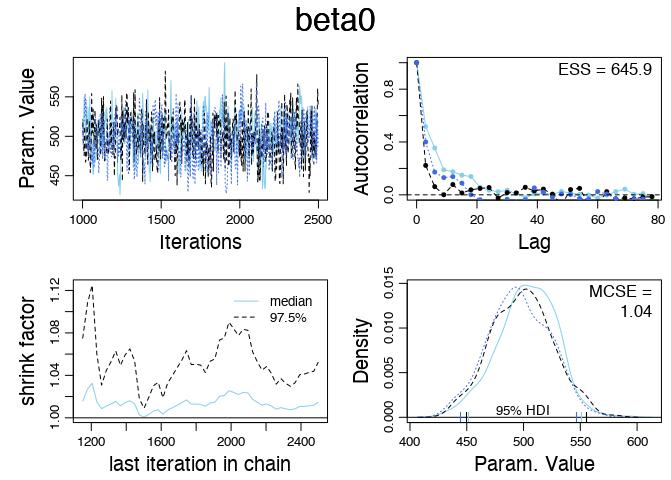
\includegraphics[width=0.5\linewidth]{/Users/ellenitoumpas/DATA/STUDY/COURSES/MASTERS-ANALYTICS/06-SEMESTER-02-2020/MATH2269_APPLIED_BAYESIAN_STATISTICS/FINAL_PROJECT/bayesian-final-project/OUTPUTS/IMAGES/BETA_DIAGNOSTICS/MODEL_001_GAMMA_GAMMA_C3_A500_B500_T3/model_001_gamma_gamma_c3_a500_b500_t3_namesDiagbeta0} 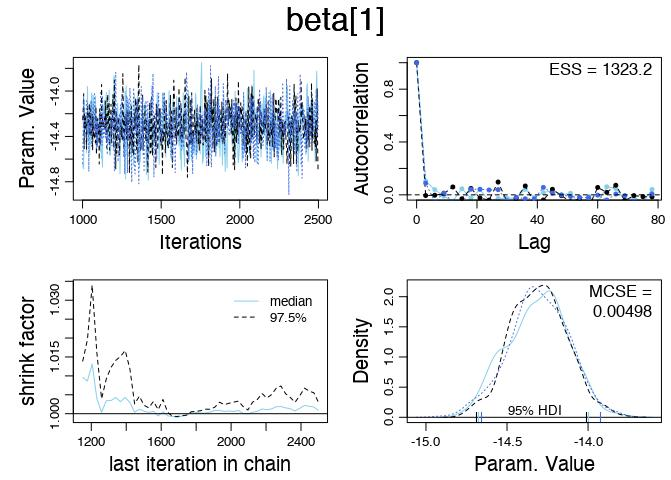
\includegraphics[width=0.5\linewidth]{/Users/ellenitoumpas/DATA/STUDY/COURSES/MASTERS-ANALYTICS/06-SEMESTER-02-2020/MATH2269_APPLIED_BAYESIAN_STATISTICS/FINAL_PROJECT/bayesian-final-project/OUTPUTS/IMAGES/BETA_DIAGNOSTICS/MODEL_001_GAMMA_GAMMA_C3_A500_B500_T3/model_001_gamma_gamma_c3_a500_b500_t3_namesDiagbeta[1]} 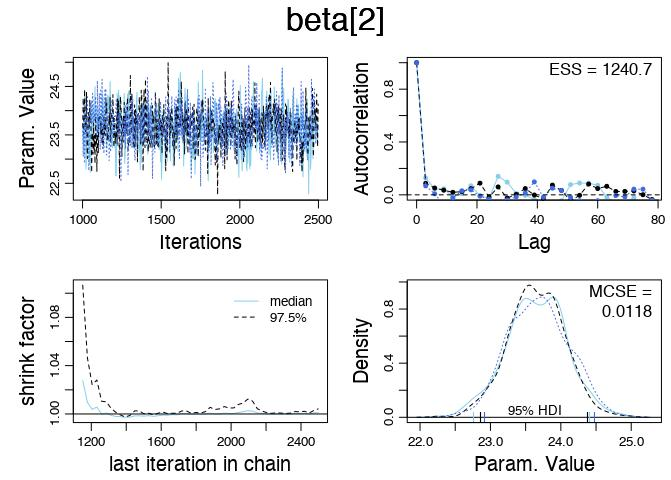
\includegraphics[width=0.5\linewidth]{/Users/ellenitoumpas/DATA/STUDY/COURSES/MASTERS-ANALYTICS/06-SEMESTER-02-2020/MATH2269_APPLIED_BAYESIAN_STATISTICS/FINAL_PROJECT/bayesian-final-project/OUTPUTS/IMAGES/BETA_DIAGNOSTICS/MODEL_001_GAMMA_GAMMA_C3_A500_B500_T3/model_001_gamma_gamma_c3_a500_b500_t3_namesDiagbeta[2]} 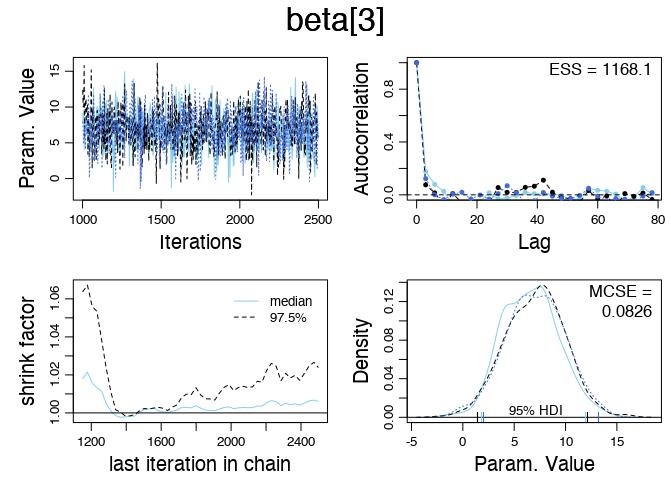
\includegraphics[width=0.5\linewidth]{/Users/ellenitoumpas/DATA/STUDY/COURSES/MASTERS-ANALYTICS/06-SEMESTER-02-2020/MATH2269_APPLIED_BAYESIAN_STATISTICS/FINAL_PROJECT/bayesian-final-project/OUTPUTS/IMAGES/BETA_DIAGNOSTICS/MODEL_001_GAMMA_GAMMA_C3_A500_B500_T3/model_001_gamma_gamma_c3_a500_b500_t3_namesDiagbeta[3]} 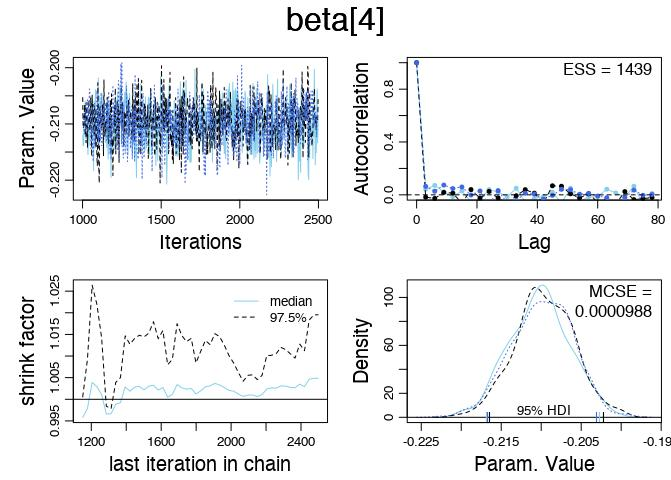
\includegraphics[width=0.5\linewidth]{/Users/ellenitoumpas/DATA/STUDY/COURSES/MASTERS-ANALYTICS/06-SEMESTER-02-2020/MATH2269_APPLIED_BAYESIAN_STATISTICS/FINAL_PROJECT/bayesian-final-project/OUTPUTS/IMAGES/BETA_DIAGNOSTICS/MODEL_001_GAMMA_GAMMA_C3_A500_B500_T3/model_001_gamma_gamma_c3_a500_b500_t3_namesDiagbeta[4]} 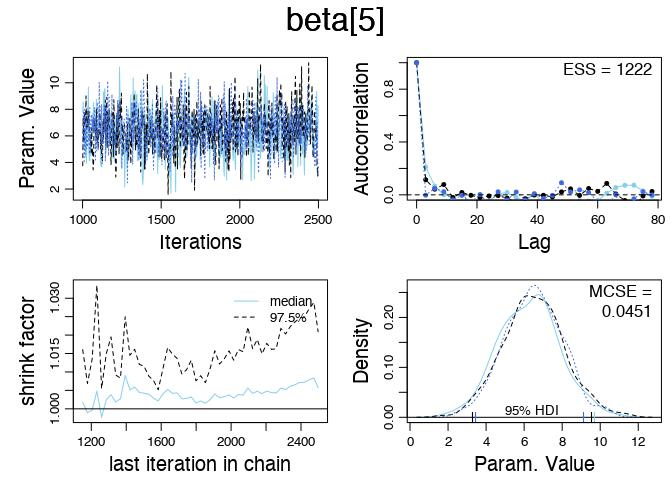
\includegraphics[width=0.5\linewidth]{/Users/ellenitoumpas/DATA/STUDY/COURSES/MASTERS-ANALYTICS/06-SEMESTER-02-2020/MATH2269_APPLIED_BAYESIAN_STATISTICS/FINAL_PROJECT/bayesian-final-project/OUTPUTS/IMAGES/BETA_DIAGNOSTICS/MODEL_001_GAMMA_GAMMA_C3_A500_B500_T3/model_001_gamma_gamma_c3_a500_b500_t3_namesDiagbeta[5]} 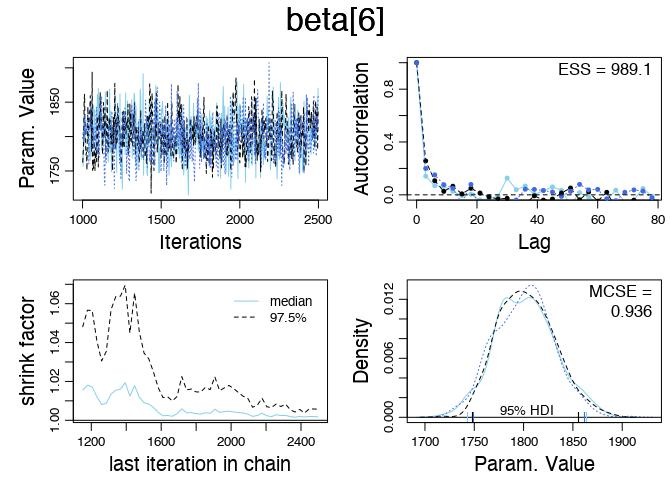
\includegraphics[width=0.5\linewidth]{/Users/ellenitoumpas/DATA/STUDY/COURSES/MASTERS-ANALYTICS/06-SEMESTER-02-2020/MATH2269_APPLIED_BAYESIAN_STATISTICS/FINAL_PROJECT/bayesian-final-project/OUTPUTS/IMAGES/BETA_DIAGNOSTICS/MODEL_001_GAMMA_GAMMA_C3_A500_B500_T3/model_001_gamma_gamma_c3_a500_b500_t3_namesDiagbeta[6]} 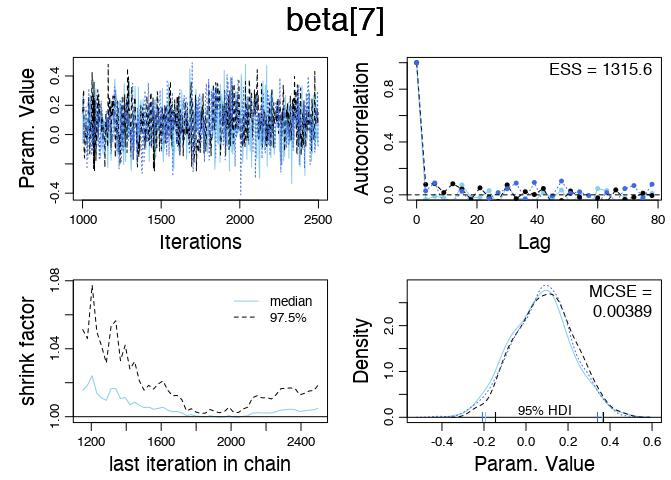
\includegraphics[width=0.5\linewidth]{/Users/ellenitoumpas/DATA/STUDY/COURSES/MASTERS-ANALYTICS/06-SEMESTER-02-2020/MATH2269_APPLIED_BAYESIAN_STATISTICS/FINAL_PROJECT/bayesian-final-project/OUTPUTS/IMAGES/BETA_DIAGNOSTICS/MODEL_001_GAMMA_GAMMA_C3_A500_B500_T3/model_001_gamma_gamma_c3_a500_b500_t3_namesDiagbeta[7]} 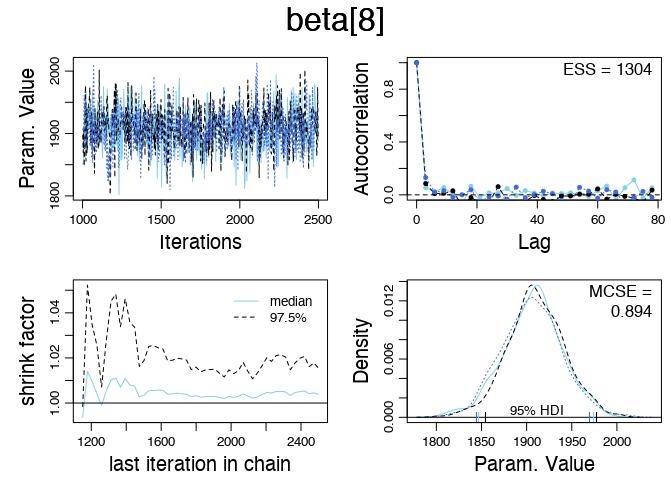
\includegraphics[width=0.5\linewidth]{/Users/ellenitoumpas/DATA/STUDY/COURSES/MASTERS-ANALYTICS/06-SEMESTER-02-2020/MATH2269_APPLIED_BAYESIAN_STATISTICS/FINAL_PROJECT/bayesian-final-project/OUTPUTS/IMAGES/BETA_DIAGNOSTICS/MODEL_001_GAMMA_GAMMA_C3_A500_B500_T3/model_001_gamma_gamma_c3_a500_b500_t3_namesDiagbeta[8]} 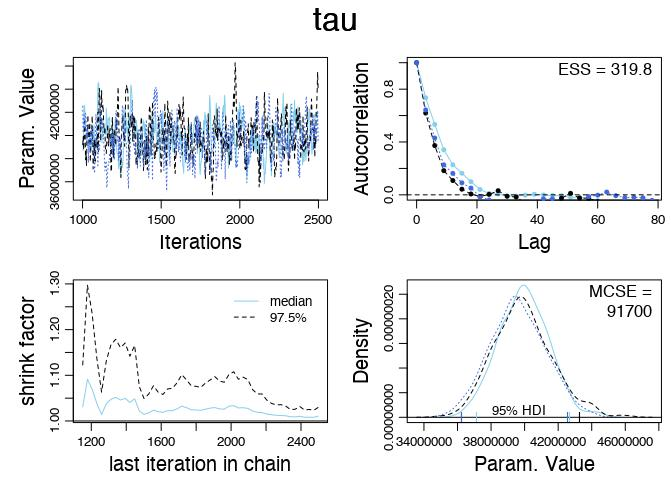
\includegraphics[width=0.5\linewidth]{/Users/ellenitoumpas/DATA/STUDY/COURSES/MASTERS-ANALYTICS/06-SEMESTER-02-2020/MATH2269_APPLIED_BAYESIAN_STATISTICS/FINAL_PROJECT/bayesian-final-project/OUTPUTS/IMAGES/BETA_DIAGNOSTICS/MODEL_001_GAMMA_GAMMA_C3_A500_B500_T3/model_001_gamma_gamma_c3_a500_b500_t3_namesDiagtau} \end{figure}

\begin{figure}[H]
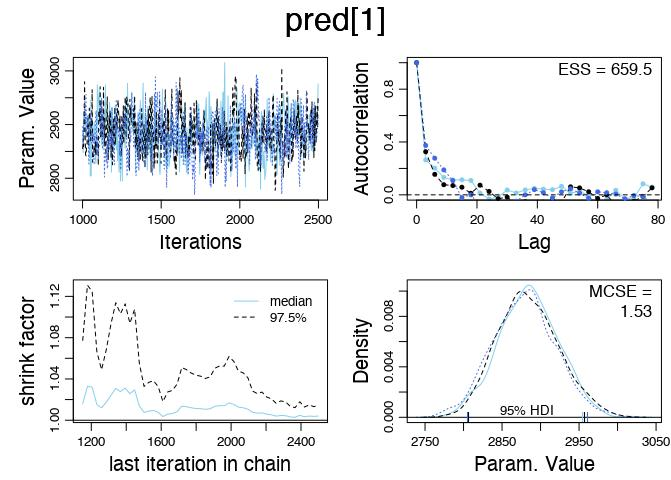
\includegraphics[width=0.5\linewidth]{/Users/ellenitoumpas/DATA/STUDY/COURSES/MASTERS-ANALYTICS/06-SEMESTER-02-2020/MATH2269_APPLIED_BAYESIAN_STATISTICS/FINAL_PROJECT/bayesian-final-project/OUTPUTS/IMAGES/BETA_DIAGNOSTICS/MODEL_001_GAMMA_GAMMA_C3_A500_B500_T3/model_001_gamma_gamma_c3_a500_b500_t3_namesDiagpred[1]} 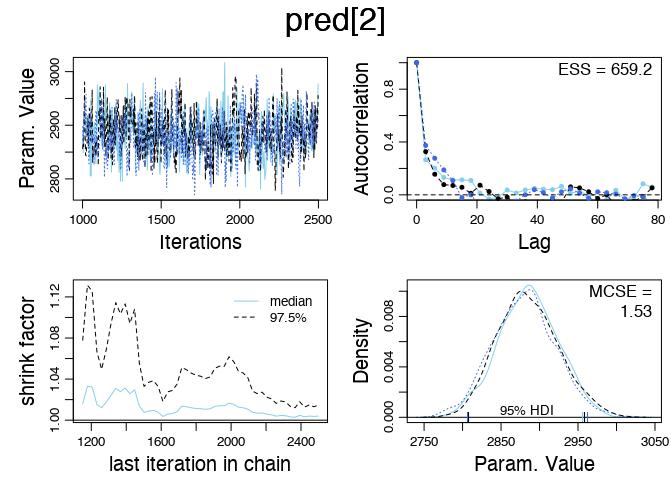
\includegraphics[width=0.5\linewidth]{/Users/ellenitoumpas/DATA/STUDY/COURSES/MASTERS-ANALYTICS/06-SEMESTER-02-2020/MATH2269_APPLIED_BAYESIAN_STATISTICS/FINAL_PROJECT/bayesian-final-project/OUTPUTS/IMAGES/BETA_DIAGNOSTICS/MODEL_001_GAMMA_GAMMA_C3_A500_B500_T3/model_001_gamma_gamma_c3_a500_b500_t3_namesDiagpred[2]} 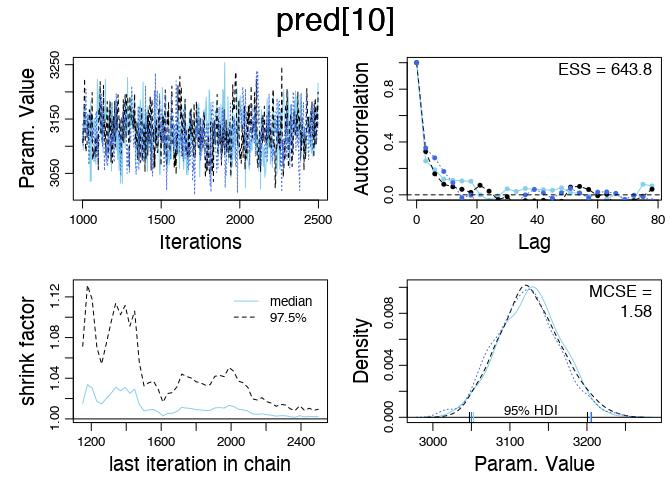
\includegraphics[width=0.5\linewidth]{/Users/ellenitoumpas/DATA/STUDY/COURSES/MASTERS-ANALYTICS/06-SEMESTER-02-2020/MATH2269_APPLIED_BAYESIAN_STATISTICS/FINAL_PROJECT/bayesian-final-project/OUTPUTS/IMAGES/BETA_DIAGNOSTICS/MODEL_001_GAMMA_GAMMA_C3_A500_B500_T3/model_001_gamma_gamma_c3_a500_b500_t3_namesDiagpred[10]} 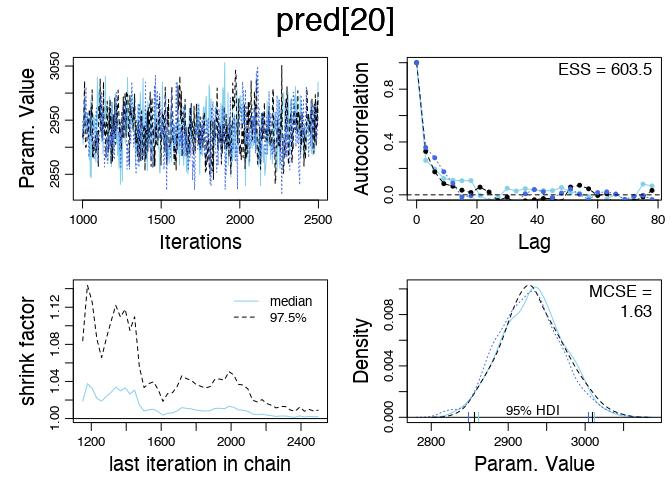
\includegraphics[width=0.5\linewidth]{/Users/ellenitoumpas/DATA/STUDY/COURSES/MASTERS-ANALYTICS/06-SEMESTER-02-2020/MATH2269_APPLIED_BAYESIAN_STATISTICS/FINAL_PROJECT/bayesian-final-project/OUTPUTS/IMAGES/BETA_DIAGNOSTICS/MODEL_001_GAMMA_GAMMA_C3_A500_B500_T3/model_001_gamma_gamma_c3_a500_b500_t3_namesDiagpred[20]} 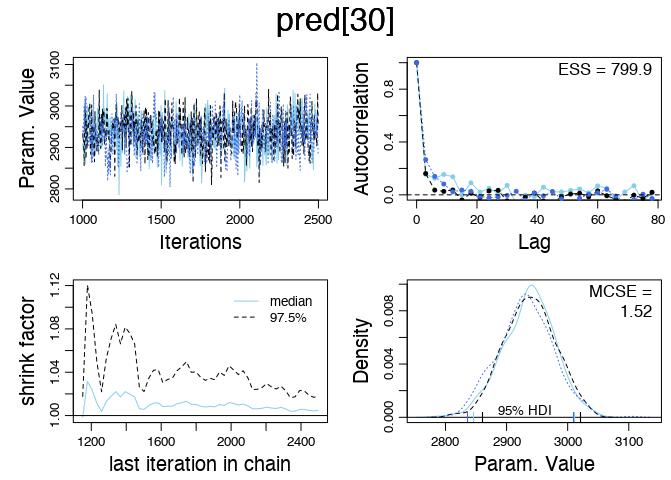
\includegraphics[width=0.5\linewidth]{/Users/ellenitoumpas/DATA/STUDY/COURSES/MASTERS-ANALYTICS/06-SEMESTER-02-2020/MATH2269_APPLIED_BAYESIAN_STATISTICS/FINAL_PROJECT/bayesian-final-project/OUTPUTS/IMAGES/BETA_DIAGNOSTICS/MODEL_001_GAMMA_GAMMA_C3_A500_B500_T3/model_001_gamma_gamma_c3_a500_b500_t3_namesDiagpred[30]} 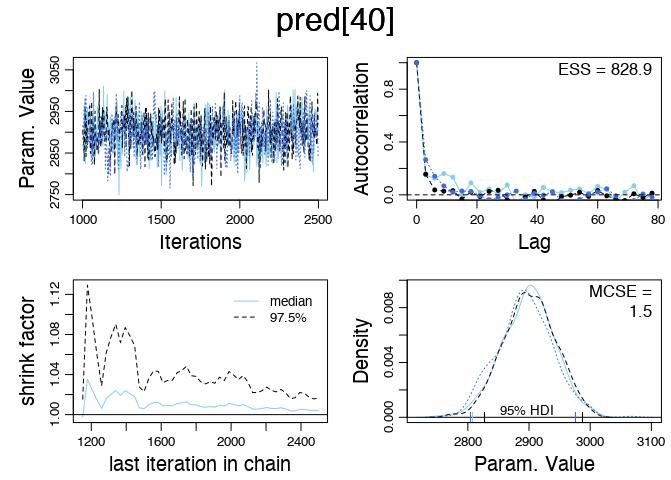
\includegraphics[width=0.5\linewidth]{/Users/ellenitoumpas/DATA/STUDY/COURSES/MASTERS-ANALYTICS/06-SEMESTER-02-2020/MATH2269_APPLIED_BAYESIAN_STATISTICS/FINAL_PROJECT/bayesian-final-project/OUTPUTS/IMAGES/BETA_DIAGNOSTICS/MODEL_001_GAMMA_GAMMA_C3_A500_B500_T3/model_001_gamma_gamma_c3_a500_b500_t3_namesDiagpred[40]} 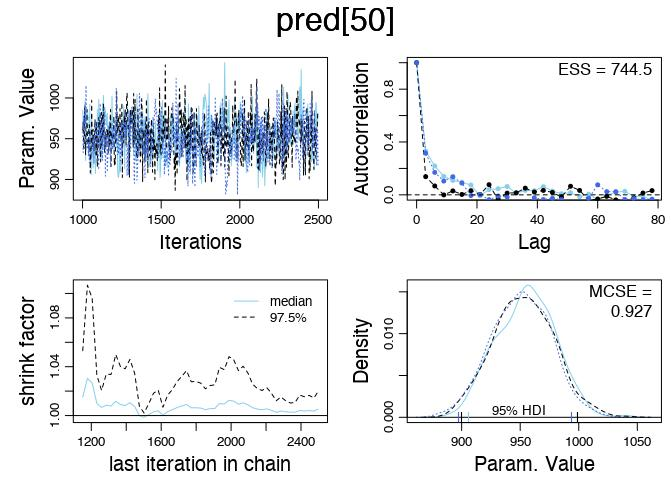
\includegraphics[width=0.5\linewidth]{/Users/ellenitoumpas/DATA/STUDY/COURSES/MASTERS-ANALYTICS/06-SEMESTER-02-2020/MATH2269_APPLIED_BAYESIAN_STATISTICS/FINAL_PROJECT/bayesian-final-project/OUTPUTS/IMAGES/BETA_DIAGNOSTICS/MODEL_001_GAMMA_GAMMA_C3_A500_B500_T3/model_001_gamma_gamma_c3_a500_b500_t3_namesDiagpred[50]} 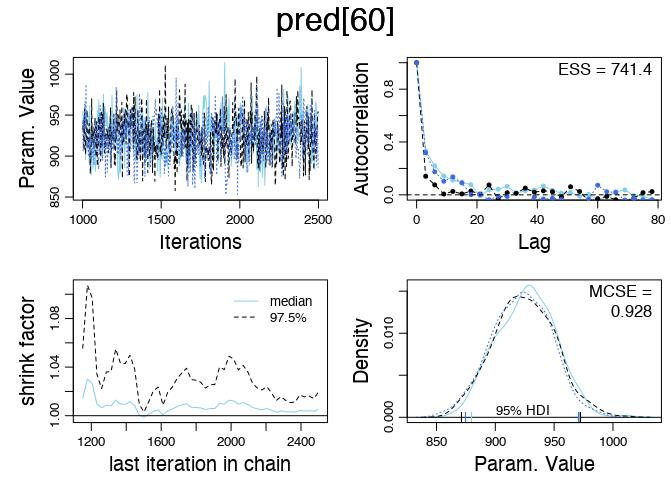
\includegraphics[width=0.5\linewidth]{/Users/ellenitoumpas/DATA/STUDY/COURSES/MASTERS-ANALYTICS/06-SEMESTER-02-2020/MATH2269_APPLIED_BAYESIAN_STATISTICS/FINAL_PROJECT/bayesian-final-project/OUTPUTS/IMAGES/BETA_DIAGNOSTICS/MODEL_001_GAMMA_GAMMA_C3_A500_B500_T3/model_001_gamma_gamma_c3_a500_b500_t3_namesDiagpred[60]} 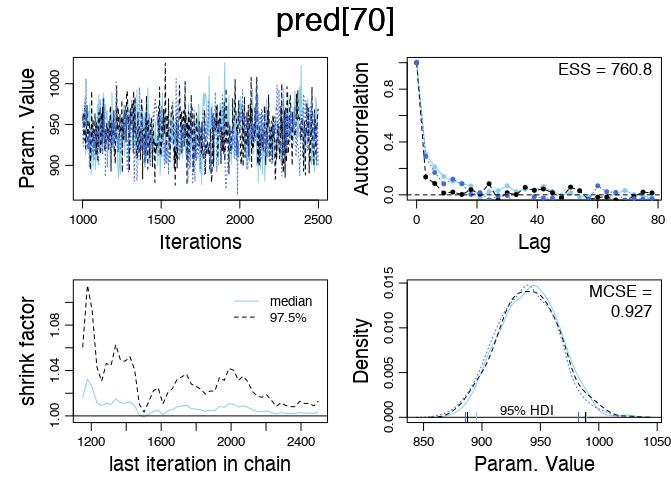
\includegraphics[width=0.5\linewidth]{/Users/ellenitoumpas/DATA/STUDY/COURSES/MASTERS-ANALYTICS/06-SEMESTER-02-2020/MATH2269_APPLIED_BAYESIAN_STATISTICS/FINAL_PROJECT/bayesian-final-project/OUTPUTS/IMAGES/BETA_DIAGNOSTICS/MODEL_001_GAMMA_GAMMA_C3_A500_B500_T3/model_001_gamma_gamma_c3_a500_b500_t3_namesDiagpred[70]} \end{figure}

\begin{Shaded}
\begin{Highlighting}[]
\KeywordTok{view_summary_table}\NormalTok{(trial_type) }\OperatorTok\StringTok{ }
\StringTok{  }\KeywordTok{format_table}\NormalTok{(}\DataTypeTok{p_caption=}\StringTok{""}\NormalTok{)}
\end{Highlighting}
\end{Shaded}

\begin{table}

\caption{\label{tab:unnamed-chunk-31}}
\centering
\begin{tabu} to \linewidth {>{\raggedright}X>{\raggedleft}X>{\raggedleft}X>{\raggedleft}X>{\raggedleft}X>{\raggedleft}X>{\raggedleft}X>{\raggedleft}X>{\raggedright}X>{\raggedright}X>{\raggedright}X>{\raggedright}X>{\raggedright}X>{\raggedright}X>{\raggedright}X}
\hline
X & Mean & Median & Mode & ESS & HDImass & HDIlow & HDIhigh & CompVal & PcntGtCompVal & ROPElow & ROPEhigh & PcntLtROPE & PcntInROPE & PcntGtROPE\\
\hline
CHAIN & 2.0000000 & 2.0000000 & 3.0022676 & 1.5 & 0.95 & 1.0000000 & 3.000000 & NA & NA & NA & NA & NA & NA & NA\\
\hline
beta0 & 499.2639740 & 499.3360000 & 497.9185555 & 465.8 & 0.95 & 447.1800000 & 551.568000 & NA & NA & NA & NA & NA & NA & NA\\
\hline
beta[1] & -14.3071228 & -14.3061500 & -14.2497131 & 1305.1 & 0.95 & -14.6599000 & -13.953800 & NA & NA & NA & NA & NA & NA & NA\\
\hline
beta[2] & 23.6630136 & 23.6566500 & 23.5529786 & 1237.8 & 0.95 & 22.8543000 & 24.460400 & NA & NA & NA & NA & NA & NA & NA\\
\hline
beta[3] & 6.8977872 & 6.9475500 & 7.7574681 & 1161.6 & 0.95 & 1.4180300 & 12.136000 & NA & NA & NA & NA & NA & NA & NA\\
\hline
beta[4] & -0.2098892 & -0.2098835 & -0.2103907 & 1500.0 & 0.95 & -0.2168640 & -0.202666 & NA & NA & NA & NA & NA & NA & NA\\
\hline
beta[5] & 6.4216764 & 6.4567950 & 6.6406596 & 1080.9 & 0.95 & 3.4291200 & 9.594490 & NA & NA & NA & NA & NA & NA & NA\\
\hline
beta[6] & 1801.7689333 & 1801.2900000 & 1805.7142746 & 867.3 & 0.95 & 1745.7700000 & 1859.940000 & NA & NA & NA & NA & NA & NA & NA\\
\hline
beta[7] & 0.0794385 & 0.0834228 & 0.0997201 & 1269.0 & 0.95 & -0.1886320 & 0.355125 & NA & NA & NA & NA & NA & NA & NA\\
\hline
beta[8] & 1907.6886933 & 1908.0200000 & 1907.3549178 & 1243.0 & 0.95 & 1849.7900000 & 1976.940000 & NA & NA & NA & NA & NA & NA & NA\\
\hline
zbeta0 & 24.9263915 & 24.9300000 & 24.8592012 & 465.8 & 0.95 & 22.3260000 & 27.537800 & NA & NA & NA & NA & NA & NA & NA\\
\hline
zbeta[1] & -5.3207371 & -5.3203650 & -5.2993750 & 1305.1 & 0.95 & -5.4519400 & -5.189340 & NA & NA & NA & NA & NA & NA & NA\\
\hline
zbeta[2] & 6.9852882 & 6.9834100 & 6.9528096 & 1237.8 & 0.95 & 6.7465500 & 7.220680 & NA & NA & NA & NA & NA & NA & NA\\
\hline
zbeta[3] & 0.5018392 & 0.5054595 & 0.5643846 & 1161.6 & 0.95 & 0.1031670 & 0.882936 & NA & NA & NA & NA & NA & NA & NA\\
\hline
zbeta[4] & -0.6467360 & -0.6467185 & -0.6482804 & 1500.0 & 0.95 & -0.6682290 & -0.624481 & NA & NA & NA & NA & NA & NA & NA\\
\hline
zbeta[5] & 0.6412128 & 0.6447195 & 0.6630789 & 1080.9 & 0.95 & 0.3424020 & 0.958023 & NA & NA & NA & NA & NA & NA & NA\\
\hline
zbeta[6] & 40.5845967 & 40.5738000 & 40.6733946 & 867.3 & 0.95 & 39.3232000 & 41.894800 & NA & NA & NA & NA & NA & NA & NA\\
\hline
zbeta[7] & 0.0268893 & 0.0282380 & 0.0337544 & 1269.0 & 0.95 & -0.0638505 & 0.120207 & NA & NA & NA & NA & NA & NA & NA\\
\hline
zbeta[8] & 41.7980944 & 41.8052500 & 41.7908303 & 1243.0 & 0.95 & 40.5295000 & 43.315500 & NA & NA & NA & NA & NA & NA & NA\\
\hline
tau & 39822823.8000000 & 39765650.0000000 & 39698357.7560163 & 312.1 & 0.95 & 36360400.0000000 & 42754800.000000 & NA & NA & NA & NA & NA & NA & NA\\
\hline
zVar & 99263.6963333 & 99121.1000000 & 98953.4644451 & 312.1 & 0.95 & 90633.2000000 & 106572.000000 & NA & NA & NA & NA & NA & NA & NA\\
\hline
pred[1] & 2882.4102067 & 2882.2300000 & 2883.7895721 & 549.3 & 0.95 & 2804.0500000 & 2956.490000 & NA & NA & NA & NA & NA & NA & NA\\
\hline
pred[2] & 2883.6339467 & 2883.5100000 & 2885.0730600 & 548.7 & 0.95 & 2805.5900000 & 2957.920000 & NA & NA & NA & NA & NA & NA & NA\\
\hline
pred[10] & 3124.8543667 & 3124.7050000 & 3124.9200590 & 604.4 & 0.95 & 3050.1000000 & 3203.970000 & NA & NA & NA & NA & NA & NA & NA\\
\hline
pred[20] & 2930.5344400 & 2930.3100000 & 2932.0561737 & 592.5 & 0.95 & 2854.9400000 & 3008.070000 & NA & NA & NA & NA & NA & NA & NA\\
\hline
pred[30] & 2935.2638533 & 2936.1700000 & 2935.9509523 & 713.1 & 0.95 & 2847.5900000 & 3015.700000 & NA & NA & NA & NA & NA & NA & NA\\
\hline
pred[40] & 2897.8973867 & 2898.0550000 & 2894.9128228 & 772.8 & 0.95 & 2809.4400000 & 2976.630000 & NA & NA & NA & NA & NA & NA & NA\\
\hline
pred[50] & 952.8020907 & 953.4195000 & 954.7756295 & 612.1 & 0.95 & 902.3930000 & 999.600000 & NA & NA & NA & NA & NA & NA & NA\\
\hline
pred[60] & 924.3415613 & 924.8925000 & 926.7147427 & 608.4 & 0.95 & 874.4610000 & 972.168000 & NA & NA & NA & NA & NA & NA & NA\\
\hline
pred[70] & 939.5203053 & 939.7135000 & 941.1702871 & 636.5 & 0.95 & 888.6290000 & 987.090000 & NA & NA & NA & NA & NA & NA & NA\\
\hline
\end{tabu}
\end{table}

\begin{figure}[H]
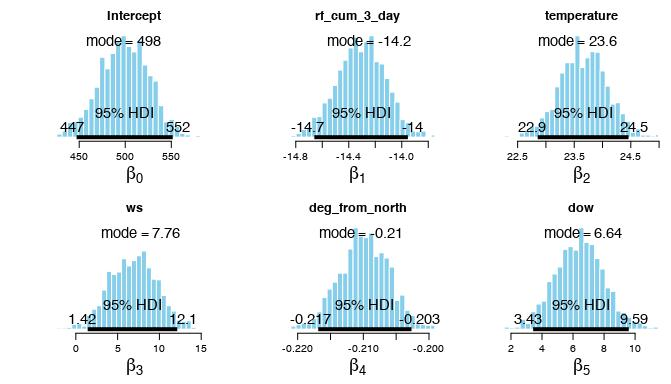
\includegraphics[width=0.5\linewidth]{/Users/ellenitoumpas/DATA/STUDY/COURSES/MASTERS-ANALYTICS/06-SEMESTER-02-2020/MATH2269_APPLIED_BAYESIAN_STATISTICS/FINAL_PROJECT/bayesian-final-project/OUTPUTS/IMAGES/POSTERIOR_DIAGNOSTICS/MODEL_001_GAMMA_GAMMA_C3_A500_B500_T3/model_001_gamma_gamma_c3_a500_b500_t3Post_Beta1} 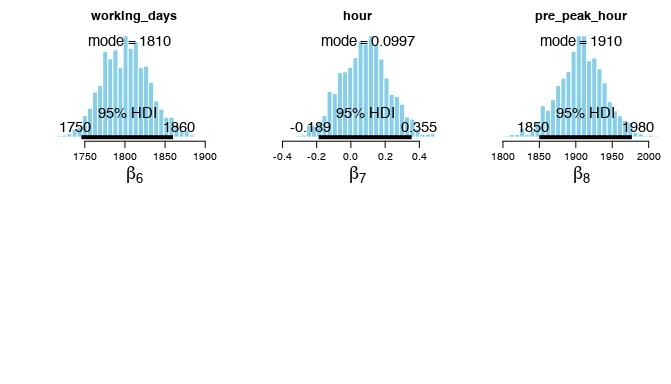
\includegraphics[width=0.5\linewidth]{/Users/ellenitoumpas/DATA/STUDY/COURSES/MASTERS-ANALYTICS/06-SEMESTER-02-2020/MATH2269_APPLIED_BAYESIAN_STATISTICS/FINAL_PROJECT/bayesian-final-project/OUTPUTS/IMAGES/POSTERIOR_DIAGNOSTICS/MODEL_001_GAMMA_GAMMA_C3_A500_B500_T3/model_001_gamma_gamma_c3_a500_b500_t3Post_Beta2} 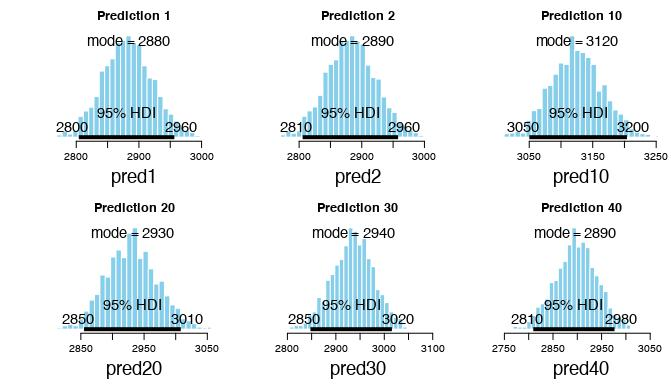
\includegraphics[width=0.5\linewidth]{/Users/ellenitoumpas/DATA/STUDY/COURSES/MASTERS-ANALYTICS/06-SEMESTER-02-2020/MATH2269_APPLIED_BAYESIAN_STATISTICS/FINAL_PROJECT/bayesian-final-project/OUTPUTS/IMAGES/POSTERIOR_DIAGNOSTICS/MODEL_001_GAMMA_GAMMA_C3_A500_B500_T3/model_001_gamma_gamma_c3_a500_b500_t3Post_Pred1} 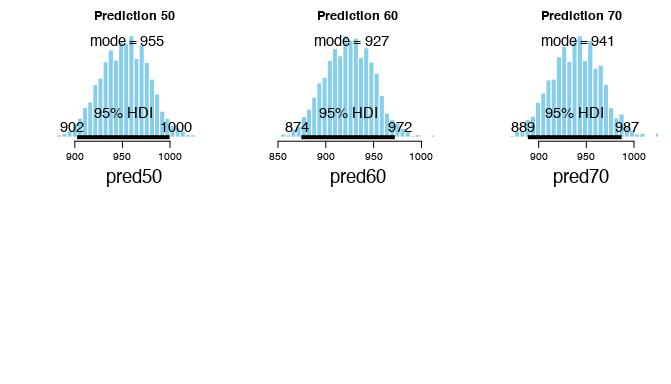
\includegraphics[width=0.5\linewidth]{/Users/ellenitoumpas/DATA/STUDY/COURSES/MASTERS-ANALYTICS/06-SEMESTER-02-2020/MATH2269_APPLIED_BAYESIAN_STATISTICS/FINAL_PROJECT/bayesian-final-project/OUTPUTS/IMAGES/POSTERIOR_DIAGNOSTICS/MODEL_001_GAMMA_GAMMA_C3_A500_B500_T3/model_001_gamma_gamma_c3_a500_b500_t3Post_Pred2} 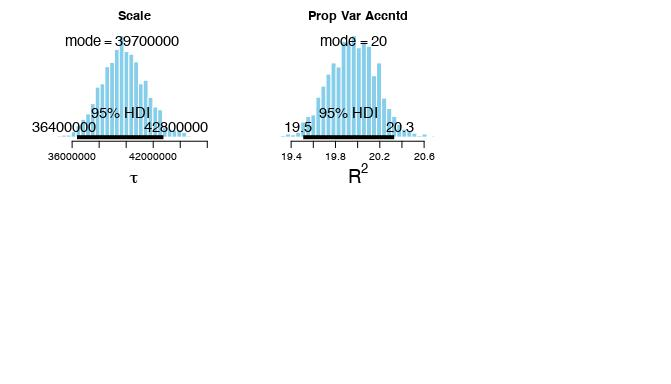
\includegraphics[width=0.5\linewidth]{/Users/ellenitoumpas/DATA/STUDY/COURSES/MASTERS-ANALYTICS/06-SEMESTER-02-2020/MATH2269_APPLIED_BAYESIAN_STATISTICS/FINAL_PROJECT/bayesian-final-project/OUTPUTS/IMAGES/POSTERIOR_DIAGNOSTICS/MODEL_001_GAMMA_GAMMA_C3_A500_B500_T3/model_001_gamma_gamma_c3_a500_b500_t3PostMarg1} 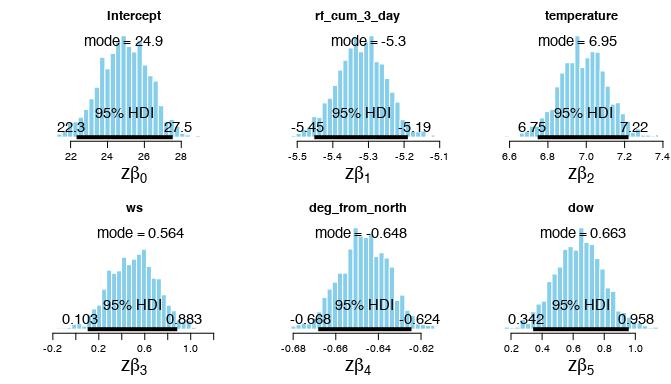
\includegraphics[width=0.5\linewidth]{/Users/ellenitoumpas/DATA/STUDY/COURSES/MASTERS-ANALYTICS/06-SEMESTER-02-2020/MATH2269_APPLIED_BAYESIAN_STATISTICS/FINAL_PROJECT/bayesian-final-project/OUTPUTS/IMAGES/POSTERIOR_DIAGNOSTICS/MODEL_001_GAMMA_GAMMA_C3_A500_B500_T3/model_001_gamma_gamma_c3_a500_b500_t3PostMargZ1} 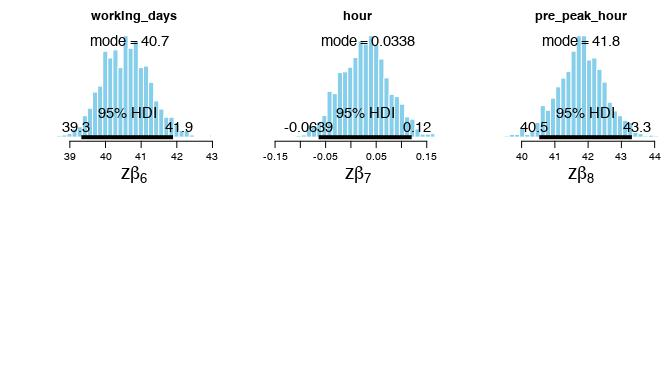
\includegraphics[width=0.5\linewidth]{/Users/ellenitoumpas/DATA/STUDY/COURSES/MASTERS-ANALYTICS/06-SEMESTER-02-2020/MATH2269_APPLIED_BAYESIAN_STATISTICS/FINAL_PROJECT/bayesian-final-project/OUTPUTS/IMAGES/POSTERIOR_DIAGNOSTICS/MODEL_001_GAMMA_GAMMA_C3_A500_B500_T3/model_001_gamma_gamma_c3_a500_b500_t3PostMargZ2} 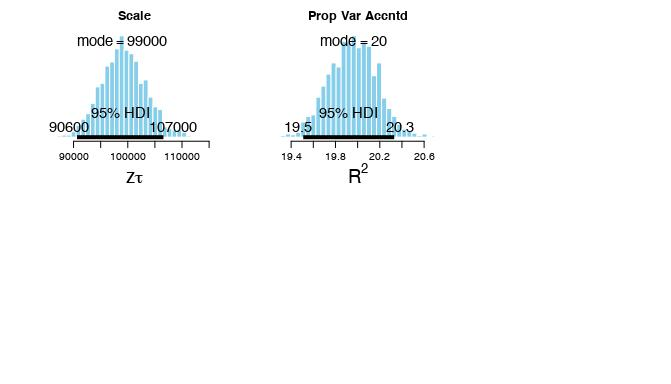
\includegraphics[width=0.5\linewidth]{/Users/ellenitoumpas/DATA/STUDY/COURSES/MASTERS-ANALYTICS/06-SEMESTER-02-2020/MATH2269_APPLIED_BAYESIAN_STATISTICS/FINAL_PROJECT/bayesian-final-project/OUTPUTS/IMAGES/POSTERIOR_DIAGNOSTICS/MODEL_001_GAMMA_GAMMA_C3_A500_B500_T3/model_001_gamma_gamma_c3_a500_b500_t3PostMargZ21} \end{figure}

\hypertarget{experiments-to-improve-model-efficiency}{%
\subsubsection{Experiments to improve model
efficiency}\label{experiments-to-improve-model-efficiency}}

\hypertarget{isolated-experiments-on-adapt-steps}{%
\paragraph{Isolated experiments on adapt
steps}\label{isolated-experiments-on-adapt-steps}}

\hypertarget{isolated-experiments-on-burn-in-steps}{%
\paragraph{Isolated experiments on burn in
steps}\label{isolated-experiments-on-burn-in-steps}}

\hypertarget{isolated-experiments-on-thinning-steps}{%
\paragraph{Isolated experiments on thinning
steps}\label{isolated-experiments-on-thinning-steps}}

\hypertarget{isolated-experiments-on-number-of-saved-steps}{%
\paragraph{Isolated experiments on number of saved
steps}\label{isolated-experiments-on-number-of-saved-steps}}

\hypertarget{isolated-experiments-with-initial-values}{%
\paragraph{Isolated experiments with initial
values}\label{isolated-experiments-with-initial-values}}

\hypertarget{model-fine-tuning}{%
\subsubsection{Model fine-tuning}\label{model-fine-tuning}}

\hypertarget{prior-sensitivity-analysis}{%
\subsubsection{Prior sensitivity
analysis}\label{prior-sensitivity-analysis}}

\hypertarget{posterior-inferences}{%
\subsubsection{Posterior Inferences}\label{posterior-inferences}}

\hypertarget{results}{%
\subsubsection{Results}\label{results}}

\hypertarget{prediction}{%
\subsubsection{Prediction}\label{prediction}}

\hypertarget{conclusion}{%
\subsection{Conclusion}\label{conclusion}}

\hypertarget{reference}{%
\subsection{Reference}\label{reference}}

\hypertarget{appendix}{%
\subsection{Appendix}\label{appendix}}

\bibliographystyle{agsm}
\bibliography{bibliography.bib}

\end{document}
